
\chapter{自指和自复制}

在这一章里,我们要看看导致各种自指现象的机制,并把它们与一些使某几种系统能够复制自己的技巧加以比较。我们将展现这些技巧之间的一些值得注意的、漂亮的相似性。

\section{隐性和显性的自指句子}

作为开篇,我们先看几个句子,这些句子第一眼看去像是最简单的自指。下面是这一类句子中的几个例子:
\begin{enumerate}
\item 本句子有七个字。
\item 本句子无意义,因为它是自指的。
\item 本句子无动词。
\item 本句子是假的。\lnote{(说谎者悖论)}
\item 正在写的这句话就是你正在读的那句话。
\end{enumerate}
除了最后一句(这是个例外),其余的所有句子都涉及一个看上去很简单的、包含在词组“本句子”之内的技巧。其实,这种技巧一点也不简单。全部这些句子都“漂浮”在上下文之中。可以把它们与只能看见尖顶的冰山做个比较。这一串串字符就是冰山的尖顶,为了理解它们所必须做的处理就是看不见的那部分。按这种意义,它们的涵义是隐性的,而不是显性的。当然,没有一句话的意义完全是显性的,不过,这种自指性越是呈显性,就越能暴露支撑它的那种技巧。在我们这里,为了辨认出上述各句子的自指性,就不仅要熟悉像汉语这样的、可以用来讨论语言学问题的语言,而且还得能够领会“本句子”这个词组的所指。这好像很简单,但是却要依赖于我们那种非常复杂而又完全内化了的驾驭语言的能力。这里,尤其重要的一件事是领会一个带有指示代词的名词性词组的所指。这种能力建立得很慢,因而决不能等闲视之。当我们向某个不懂得悖论和语言学圈套的人(比方说一个孩子)介绍像第四句话那样的句子时,困难也许就会特别突出。他们可能会问:“什么句子是假的?”而要想使人了解这个句子是谈论它自己的,可能就得花上一些功夫。整个思想最初是有点令人吃惊的。

\begin{lrbox}{\TEMPBOX}%
\begin{tikzpicture}[semithick,every node/.style={inner sep=0mm,font=\small}]
\coordinate (O) at (0,0);
\node[anchor=south]
  (A) at (0,.3) {说谎者句子};
\node[anchor=north,align=center,font=\linespread{1}\small]
  (B) at (0,-.5){为了理解\\说谎者句子的自指性\\所必须做的认知处理};
\node[draw,line join=round,fit=(A) (B),inner ysep=5mm,
      trapezium,trapezium angle=75,decorate,
      decoration={random steps,segment length=5pt,amplitude=5pt}] (C) {};
\draw[decorate,decoration={coil,mirror,amplitude=.5mm,segment length=5mm}]
  ([xshift=-5mm]O-|C.bottom left corner) --
  ([xshift=10mm]O-|C.bottom right corner)
  node[at end,right](R){水线};
\node[below=10mm of R.east,anchor=east]{知识海洋};
\end{tikzpicture}
\end{lrbox}

\begin{figure}
\begin{floatrow}
\figurebox[\FBwidth]{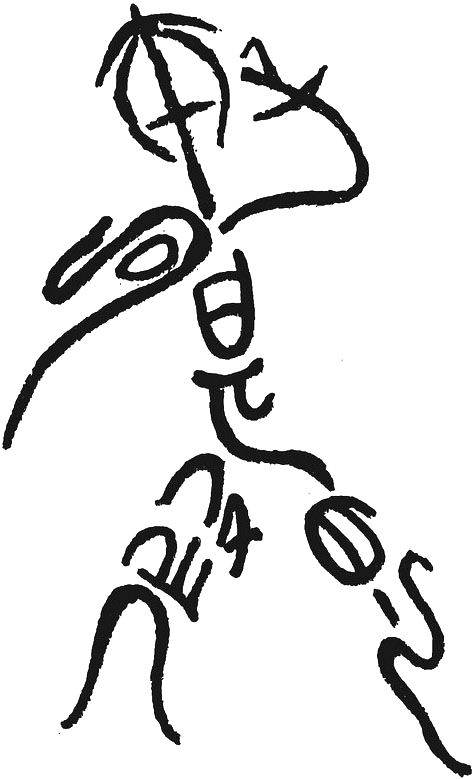
\includegraphics[height=.3\textheight]{img_083.png}}
          {\caption[说谎者处决自己。]{刘皓明绘。}}
\figurebox[\Xhsize]{\usebox\TEMPBOX}
          {\caption[说谎者悖论的冰山。]{}}
\end{floatrow}
\end{figure}

这里有两幅画(\fig{83}、\fig{84})或许会有所帮助。\fig{83}是一幅能在两个层次上解释的画。在一个层次上,它是一个指着自己的句子;在另一个层次上,它是说谎者处决自己的写照。

而为了辨认一个句子的自指性所需要的处理的相对比例,就像是\fig{84}中的冰山的可见和不可见部分的相对比例。

试着造一个自指句子,而又不用“本句子”等手法,是非常有意思的。可以试试在一个句子内部引用自己。下面就是一次尝试:

\begin{block}
“这句话有七个字”这句话有七个字。
\end{block}

不过,这种尝试必然失败,因为一个句子引用自己后得到的新句子总是比自己长。只有当你情愿接受一个无穷长的句子时,这种做法才实际可行,例如:

\begingroup
“句子\indentcr[\ccwd]\\
\small “句子\\
\footnotesize “句子\\
\scriptsize “句子\strut\\
\begin{tikzpicture}[inner sep=0pt, decoration={markings,
  mark=between positions 0 and 1 step 0.1 with
    {\fill (0,0) circle (\dimexpr 1pt * \numexpr 11 - \pgfkeysvalueof{/pgf/decoration/mark info/sequence number}\relax / 10\relax);}}]
\node[anchor=east,font=\tiny] (O) at (.6\linewidth,0) {等等,等等};
\path[postaction=decorate] (0,15mm)  to [bend right=15] (O.center);
\path[postaction=decorate] (0,-15mm) to [bend left=15]  (O.center);
\end{tikzpicture}\indentcr*\\
\scriptsize 是无穷长的”\\
\footnotesize 是无穷长的”\\
\small 是无穷长的”\\
\normalsize 是无穷长的”\par
\endgroup

但是对有穷的句子不能这样做。基于同样的理由,哥德尔的符号串G不能含有其哥德尔数的数字形式:它装不下。没有一个TNT符号串能含有其自身哥德尔数的TNT数字,因为这一数字总比该符号串本身含有更多的符号。不过,你可以让G含有其自身哥德尔数的一个描述,再利用“代入”和“算术㧟摁化”来绕过去。

蒯恩的方法是使用描述——而不是自引用或词组“本句子”——来在一个句子中实现自指的方法之一,对话《G弦上的咏叹调》里对这种方法有形象的说明。理解蒯恩句子用不着像理解前面举的四个例子那样做精巧的智力加工。虽然乍一看它好像更为诡秘,其实倒是一种更为直接的方法。蒯恩的构造在下述意义上极像哥德尔的构造:它通过描述另外一个(已经证明)同构于蒯恩句子的字符串来创造自指。对这串新字符的描述,是由这蒯恩句子的两个部分实现的。一部分是一组指令,它告诉我们如何建立一个词组,而另一部分则含有所要的素材,也就是说,这另一部分是一块模板。这也像冰山,但更像一块漂在水面上的肥皂(见\fig{85})。

\begin{figure}
%\includegraphics{img_085.png}
\begin{tikzpicture}[semithick,every node/.style={inner sep=0mm,font=\small}]
\coordinate (O) at (0,0);
\node[anchor=south]
  (A) at (0,.4) {蒯恩句子};
\node[anchor=north]
  (B) at (0,-.2){为了理解它所需的处理};
\node[draw,fit=(A) (B),inner sep=3mm,yshift=1mm,
   rounded rectangle,rounded corners,rounded rectangle arc length=90] (C) {};
\draw[decorate,decoration={coil,mirror,amplitude=.7mm,segment length=8mm}]
  ([xshift=-20mm]O-|C.west) -- ([xshift=20mm]O-|C.east)
  node[at end,right]{水线};
\end{tikzpicture}
\caption[蒯恩句子的肥皂。]
  {}
\end{figure}

这个句子的自指性是靠一种比说谎者悖论更为直接的方法达到的,用不着多少隐蔽的处理。此外,有意思的是,请注意“这个句子”出现在上面的句子里,但它在那里并不引起自指。你大约可以理解,它的所指是蒯恩句子,而不是它出现于其中的那个句子。这正好说明了诸如“这个句子”这类指示词组该如何根据上下文来解释。这还有助于说明对这种词组的处理必定是相当复杂的。

\section{一个自复制的程序}

“㧟摁化”概念以及它在制造自指过程中的用处,对话中已经解释了,所以这里用不着再细讲。我们还是来说明一下计算机程序如何能利用完全相同的技巧复制它自己。下面的自复制程序是用一种类似BlooP的语言写出的,用于在一句话之后引用它自己(这与㧟摁化次序相反,所以我把“㧟摁”倒过来写成“摁㧟”):
\begin{block}\small\raggedright
\inst{DEFINE} \inst{PROCEDURE} \inst{``ENIUQ''} $[\inst{TEMPLATE}]$: \inst{PRINT} $[$\inst{TEMPLATE}, \inst{LEFT-BRACKET}, \inst{QUOTE-MARK}, \inst{TEMPLATE}, \inst{QUOTE-MARK}, \inst{RIGHT-BRACKET}, \inst{PERIOD}$]$.

\noindent 定义过程“摁㧟”[模板]:打印[模板,左括号,单引号,模板,单引号,右括号,句号]。

\noindent \inst{ENIUQ}
\begin{block}\raggedright
\noindent\llap{$[$`}\inst{DEFINE} \inst{PROCEDURE} \inst{`ENIUQ'} $[\inst{TEMPLATE}]$: \inst{PRINT} $[$\inst{TEMPLATE}, \inst{LEFT-BRACKET}, \inst{QUOTE-MARK}, \inst{TEMPLATE}, \inst{QUOTE-MARK}, \inst{RIGHT-BRACKET}, \inst{PERIOD}$]$. \inst{ENIUQ}'$]$.
\end{block}
摁㧟
\begin{block}\raggedright
\noindent\llap{[‘}定义过程“摁㧟”[模板]:打印[模板,左括号,单引号,模板,单引号,右括号,句号]。摁㧟’]。
\end{block}
\end{block}
“\inst{ENIUQ}”是程序的前三行定义的一个过程,它的输入称作“\inst{TEMPLATE}”[模板]。这个过程的意思是:调用这个过程时,\inst{TEMPLATE}的值是某一串印刷字符,\inst{ENIUQ}的结果是执行一项打印操作,其中要把\inst{TEMPLATE}打印两次:第一次只打印它,第二次在外面加上引号和括号,最后还要缀上一个句号。这样,如果\inst{TEMPLATE}的值是符号串\inst{DOUBLE-BUBBLE}(意为“两个泡泡”),执行\inst{ENIUQ},就得到
\[
\inst{DOUBLE-BUBBLE}[\inst{`DOUBLE-BUBBLE'}]\text{。}
\]
上面的程序中,后一半是把\inst{ENIUQ}这个过程调来处理一个具体的\inst{TEMPLATE}值——即单引号内的那个长长的字串:\inst{DEFINE}\ldots\ldots\ \inst{ENIUQ}。这个值是精心挑选出来的,它由\inst{ENIUQ}的定义后面再加上一个词“\inst{ENIUQ}”组成。这就把程序本身——或者,如果你喜欢,也可以叫做程序的完全复本——给打印出来了。这很像说谎者句子的蒯恩式说法:
\begin{center}
“放在其引文形式后面得到假句子”\\
放在其引文形式后面得到假句子
\end{center}

一定要清楚,上述程序的后一半中引号内所出现的那个印刷符号串——即\inst{TEMPLATE}的值——决不能解释为一列指令。如果它碰巧是一组指令,在某种意义上,也只是巧合。如上面指出的,它同样也可以是“\inst{DOUBLE-BUBBLE}”或任何其它的印刷符号串。这个方案的出色之处在于:当同样的符号串出现在程序的前一半中时,也会被看作是一个程序(因为它不在引号之中)。因而,在这个程序中,有一个符号串以两种方式起着作用,首先是作为程序,其次是作为数据。这就是自复制程序的秘密。而且,如我们将要看到的,这也是自复制分子的秘密。顺带说一下,把任何种类的自复制的对象或自复制的实体叫做“自复制”是有益的;类似地,我们也把任何自指的对象或自指的实体称为“自指”。以后我间或要使用这些术语。

可以使用一种并非事先设计得易于书写自复制的语言来写自复制的程序,上面那个程序就是一个极好的例子。这时候,为承担起这个任务,就不得不使用一些被看作是该语言的组成部分的概念和运算——例如“\inst{QUOTE-MARK}”[引号]这个词以及“\inst{PRINT}”[打印]这个命令。但是,假如把一种语言设计得便于书写自复制,那就能写出一些很短的自复制。比方说,如果“摁㧟”运算是该语言的内在部分,而不必去做什么显式定义(就像我们对\inst{PRINT}所做的假定一样),那么,一个极其短小的自复制程序就是
\[
\inst{ENIUQ}[\inst{`ENIUQ'}]
\]
这与乌龟对蒯恩型说谎者自指句子的说法非常相似,那里要假定“㧟摁”这个动词是已知的:

\begin{block}
“被㧟摁时得到假句子”被㧟摁时得到假句子。
\end{block}

不过,自复制还能更短,比如,在某些计算机程序中可以有这样的约定:任何以星号打头的程序在正式执行前都要复制一遍。这样,这个仅由一个星号组成的程序就是一个自复制!你可能会抱怨说这很无聊,而且要依赖一个几乎完全是任意的约定。如果真是这样,那你就在重复我先前的观点:利用词组“本句子”以达到自指,几乎是个骗局——它过多地依赖处理者,而不是对自指性的直接揭示。利用一个星号做自复制的例子,就像用“我”字做自指的例子:它们都隐瞒了各自的问题中的一切令人感兴趣的方面。

这使人想起另一种新奇的自复制典型:复印机。可以断定任何手写的文件都是一个自复制,只要把它放进复印机并按一下电钮就行了。但这有点不符合我们的自复制概念。这个过程没有征求过这张纸的意见,因此它并没有指挥它自己的复制过程。于是和前面相同,所有奥妙都在处理机内。在把一个东西叫做自复制以前,我们需要有一种感觉:它应该尽可能明显的包含复制自己的方法。

确实,这种明显性是个程度问题。不过有一个直观的界限,在界限的这一边,是真正的自指挥的自复制过程,而另一边只有那种通过一台一成不变的、自动的复印机所做的复制。

\section{什么是副本?}

在对自指和自复制的任何讨论中,我们早晚都得面临“什么是副本”这个问题。在第五章和第六章中我们曾相当严肃地讨论过它,现在再来回到这个问题。为了领略这个问题的风味,我们先来看一些高度荒诞而又似乎有理的自复制例子。

\section{一首自复制的歌}

设想在一间酒吧里有一台投币式自动唱机,只要你摁一下按钮$7$,它就会放出下面这首像情歌一样的曲子:
\begin{center}
再投一枚硬币吧,放进这台投币唱机,\\
我将不断地歌唱,要的仅仅就是按$7$。
\end{center}
我们可以为此画一个小图(\fig{86}):

\begin{figure}
%\includegraphics{img_086.png}
\begin{tikzpicture}[arrow decoration]
\path[every node/.style={draw,ellipse,minimum width=15mm}]
  node (A) {歌}
  node (B) [right= 3cm of A] {\hbox{“$7$”\unskip}};
\path[auto=left,
      every node/.style={inner sep=0pt,outer sep=1.5mm},
      every edge/.style={draw,postaction=decorate,bend left}]
  (A) edge node {人} (B)
  (B) edge node {投币唱机} (A);
\end{tikzpicture}
\caption{一首自复制的歌。}
\end{figure}

尽管效果是歌曲复制了自己,但要把这首歌叫做自复制,总感到有些不对头。因为事实是,当它通过“$7$”时,全部的信息并不在那里。信息之所以得以返回,只是由于信息全部保存在自动唱机内——也就是说,是在图上的一个箭头里,并非那个椭圆内。这首歌是否包含一个有关如何使它自己被重放的完整描述,是大可怀疑的,因为“$7$”只是一个触发器,而不是一个副本。

\section{一个“螃蟹”程序}

下面来考虑一个把自己倒着打印出来的程序(某些读者可能会愿意考虑一下如何利用前面给出的那个自复制模型,用上述类似BlooP的语言写出这样一个程序)。能不能把这样一个滑稽的程序看作自复制呢?在某种意义上说是可以的。因为只要对它的输出做一个不足道的变换就能恢复原先的程序。说这个输出含有和投币唱机程序本身一样的信息,只是简单的重复,似乎也是公平的。然而很明显,某些人也可以眼看着这个输出而看不出它是个倒着打印出来的程序。回忆一下第六章的术语,我们可以说这个输出与这个程序的“内在消息”相同,不过却有不同的“外在消息”——也就是说,必须用不同的解码方式来读它们。现在,如果把外在消息看成信息的一部分——这好像十分合理——那么,全部的信息终归并不相同。所以这个程序不能算是自复制。

但是,这是一个使人不安的结论。因为我们习惯于认为一件东西和它的镜像含有相同的信息。不过,回忆一下在第六章中,我们曾使“固有意义”这一概念依赖于把智能假定为一个普遍观念。其思想是,在确定一个对象的固有意义时,我们可以忽视某些类型的外在消息——那些能够普遍被理解的信息。也就是说,在某种仍有缺陷的意义上,如果解码机制看上去足够基本,那么所要揭示的内在消息就是该考虑的唯一意义。在这个例子中,就似乎有充分的把握猜想一个“标准智能”会认为两个镜像含有彼此相同的信息。这也就是说,它认为两者之间的同构映射十分不足道,以至可以忽略。因而,我们可以认为在某种意义上,该程序算是个十足的自复制。这样的直观是站得住脚的。

\section{说谎者横跨太平洋}

自复制的另一个稀奇古怪的例子是一个打印自己的程序,不过是翻译成另一种计算机语言以后再打印。可以把它与下述古怪的蒯恩型说谎者自指的说法作个比较:
\begin{quote}
``is an expression which, when it is preceded by its translation, placed in quotation marks, into the language originating on the other side of the Pacific Ocean, yields a falsehood''是一段陈述,说的是把它译成太平洋另一侧的语言,然后再加上引号放在前面,就得到假句子。
\end{quote}

你可能要试着写写这个怪诞的混和物所描述的句子(提示:它不是它自己——或者说,至少当“它自己”取朴素的意义时,它不是它自己)。如果“逆行自复制”(即倒着写出自身的程序)的概念让人想起螃蟹卡农,那么“翻译的自复制”概念大概会使人想起带有主题转调的卡农。

\section{打印自己的哥德尔数的程序}

不打印原程序的严格副本,而打印一份译文,这种想法似乎不着边际。但是,你要是想用BlooP或FlooP写一个自复制程序,你就不得不求助于某种这样的机制,因为这些语言输出的总是一个数,而不是一个印刷符号串。所以,你只好编个程序来打印它自己的哥德尔数:一个巨大的整数,其十进展开式中每三个数字作为一个代码,一个符号一个符号地为该程序编了码。在这个程序力所能及的范围内,它已是尽其所能在打印它自己了:它打印出自己在另一个“空间”中的副本,而且,在整数空间和符号串空间之间的来回转换是很方便的。因此,输出的值不像“$7$”那样只是起一种触发作用。原程序的全部信息在输出中都是“接近表面”的。

\section{哥德尔式自指}

这已经很接近于描述哥德尔自指句子G的机制了。毕竟,那个TNT符号串不是含有一个对它自己的描述,而是含有对一个整数($u$的算术㧟摁化产物)的描述。恰巧这个整数正是符号串G在自然数空间中的一个精确的“镜像”。因此,G指向它自己在另一个空间中的翻译。称G是一个自指符号串不会感到难受,因为这两个空间之间的同构是如此严密,以致我们可以把它们看成是等同的。

把TNT反映到抽象的自然数王国里的这个同构,可以比拟成利用符号把现实世界反映到我们大脑中的那个准同构。符号对于客体充当了准同构的角色,多亏了它们,我们才能思考。类似地,哥德尔数对于符号串充当了同构的角色,多亏它们,我们才能从关于自然数的语句中找到元数学的意义。有关G的一件令人吃惊的、几乎是不可思议的事情是,它使得自指得以实现,而不理会“写出G的语言——TNT——似乎根本没有希望谈论自己的结构”这一事实。这和汉语不一样,用汉语讨论汉语是世上再容易不过的事情了。

因此,G是借助翻译达到自指的一个突出例子——但难说这是最直接的情形。也可以回过头来想想我们的某些对话,其中有些也是利用翻译达到自指的。比如,拿《无伴奏阿基里斯奏鸣曲》来说,在这篇对话里,有几处是指向巴赫的《无伴奏小提琴奏鸣曲》,而乌龟的那个建议——设想一架羽管键琴的伴奏——尤其有趣。说到底,如果把这个思想用于对话本身,就能想出乌龟说的话了;但如果假定阿基里斯部分是独立成章的(像小提琴那样),那么再把什么话归结为乌龟说的,那就十分错误了。无论如何,这里再一次有了一个利用对话到巴赫作品的映射而建立起的自指,这个映射自然就留待读者加以注意了。而且,即使读者没有注意到,映射也依然存在,对话也仍然是个自指。

\section{通过增值达到的自复制}

我们已经把自复制和卡农作了对照。那么,增值卡农的类比物该是什么呢?下面是一种可能性:考虑一个含有空循环的程序,这个循环的唯一目的是使该程序变慢,有一个参数用以指明该循环重复的频度。这样就可以作出一个打印自身的副本的自复制,不过要改变一个参量,使得当副本运行时其速度只是它的母程序的速度的一半,而它的“女儿”的速度又是它的一半,如此下去。这些程序中没有一个是严格地打印自身的,不过很明显,它们都属于同一“家族”。

这使人联想起生物的自复制过程。显然任何一个生物体都不全同于父母,那为什么生儿育女这一类事情还叫“自复制过程”呢?答案是,双亲和孩子之间有一个粗略的同构。这是一个保持物种信息的同构。因此,复制的东西是类而不是例。第五章的递归图案“G图”也是如此:在那里,不同大小和形状的“磁性蝴蝶”间的那个映射是很粗糙的。任何两个蝴蝶都不尽相同,但它们都属于同一“物种”,而这个映射恰好保持了这一事实。用自复制程序的话来说,这将与一族程序相对应,这些程序都是用出自同一种计算机语言的各种“方言”写的,每一个程序都能把自己打印出来,但都稍作改变,以使得结果是原先的语言的一种方言。

\section{凯姆式自复制}

下面的例子可能是一种最为诡秘的自复制:不是用编译语言写一个合法的表达式,而是敲进一条编译程序所使用的错误信息。当编译程序读到你的“程序”时,它一下子就会陷入混乱。因为你的“程序”不合语法,于是编译程序就打印出一个错误信息。你要做的事情,就是设法安排一下,使得它打印出来的就是你键入的那条错误信息。斯科特·凯姆向我建议的这种自复制,是利用了系统中与你通常接触的层次所不同的另一个层次。尽管看起来似乎不足道,但是,在那些各种自复制为生存而相互争斗的复杂系统中,可能会有类似的情形,这我们马上就要讨论到。

\section{什么是原件?}

除了“什么是副本”这个问题,还有一个与自复制有关的基本哲学问题,那就是上述问题的另一面:“什么是原件?”弄清这是怎么回事的最好办法是看几个例子:
\begin{enumerate}
\item 一个程序,如果用一个在计算机上运行的解释程序来解释它,它就把自己打印出来;
\item 一个程序,如果用一个在计算机上运行的解释程序来解释它,它就把自己连同该解释程序的一个完整副本(毕竟也是个程序)一起打印出来;
\item 一个程序,如果用一个在计算机上运行的解释程序来解释它,它就不仅把它自己连同该解释程序的一个完整副本都打印出来,而且还指挥着一个机械的装配过程,又装配起一部计算机,与那台运行着该程序及那个解释程序的计算机一模一样。
\end{enumerate}
很明显,在\pnum{1}中,该程序是个自复制。而在\pnum{3}中,它究竟是个自复制程序,还是程序加上解释程序的混合系统,还是程序、解释程序以及处理机的联合体呢?

显然,一个自复制可以包括比单纯地打印自己更为丰富的内容。事实上,本章余下的大部分篇幅都将用来讨论那些把数据、程序、解释程序、处理机全搅在一起的自复制,而且这种自复制会一下子把它们全都复制出来。

\section{印符遗传学}

现在,我们该讨论“生命王国的分子逻辑”这个在二十世纪最吸引人而又意义深远的课题了。这里借用了阿尔伯特·莱宁格尔富有想象力的说法。这也是逻辑——不过比人的智力所能设想的任何一种逻辑都更为复杂,也更为精彩。我们要从一个比较新颖的角度来探讨它:利用一种人工的单人游戏。我把它叫做印符遗传学。在印符遗传学里,我力图在一个印符系统(乍一看很像以"WJU"系统为代表的那类形式系统)中,捕捉分子遗传学的某些思想。当然,印符遗传学中包含了很多简化工作,从而特别有利于教学目的。

我得赶紧解释一下,分子生物学领域是一个若干层次上的各种现象相互作用的领域,而印符遗传学只打算解释来自一两个层次的现象。具体说,纯粹化学的方面完全被排除了——因为它们低于此处所讨论的层次。与此相似,古典遗传学(非分子遗传学)的一切方面也都排除在外——它们所属的层次比这里讨论的要高。我只想利用印符遗传学给出一种直观,以期说明弗兰西斯·克里克(DNA双螺旋结构的发现者之一)所阐述的、集中在著名的“分子生物学中心法则”里的那些过程:
\[
\mathrm{DNA}\Rightarrow\mathrm{RNA}\Rightarrow\text{蛋白质}
\]
我的希望是,通过我所构造的这个瘦骨伶仃的模型,读者可以了解该领域的某些简单统一的原则——否则,这些原则可能会被很多不同层次上的各种现象之间庞大而复杂的相互作用所淹没。我所牺牲的东西自然是严格的精度,所获得的东西——我希望——是一点洞见。

\section{串、基、酶}

印符遗传学游戏是在字母符号的序列上进行印符操作。要用到四个字母:
\[
\text{A\quad C\quad G\quad T}
\]
由这样四个字母组成的任意序列叫做串。下面就是一些串:
\begin{center}
GGGG\\
ATTACCA\\
CATCATCATCAT
\end{center}
顺便提一下,在印符遗传学中,串充当DNA片断的角色(在实际的遗传学中经常就把它们叫做“串”)。“信使RNA”的功能——它在印符遗传学中也用串来表示——是为DNA提供“邮政快递”服务。这将在后面看到。

有时我要把字母A、C、G、T称作基,并把它们所占据的位置称作单元。这样,上述例子中的中间那个串有七个单元,其第四个单元上放着基A。如果你有了一个串,你可以对它进行操作,用各种方式变化它。你还可以靠复制一个串或把一个串切成两半而多造出一些串。某些操作使串变长,某些使其变短,还有一些不涉及串的长度。

操作可以集束进行,也就是几项操作按次序接续执行。这样的一束操作有点像一台程序化的机器在串上移来移去地施加操作。这些活动着的机器就叫做“印符酶”——简称酶。酶在串上每次作用于一个单元,我们把这说成是酶“拴”在此刻所作用的那个单元上。

下面谈谈酶(任选几个)如何作用在具体的符号串上。首先该知道的事情是:每一种酶总喜欢一开始拴在某个特殊的字母上。所以就有四种酶——喜欢A的酶、喜欢C的酶、等等。给出某个酶执行的一系列操作之后,你就可以判断出它喜欢哪个字母了。不过现在我就给出它们,不加解释。下面是一个任选的酶,它由三项操作组成:
\begin{enumerate}
\item 删除拴着这个酶的单元(并把酶拴在右方的下一个单元上)。
\item 向右移一个单元。
\item (紧挨着这个单元,在右边)插进一个T。
\end{enumerate}
这个酶正巧是喜欢一开始拴在A上的。我们用下面这个串作样本,看看酶怎么工作:
\[
\text{ACA}
\]
如果我们的酶拴在左边的A上并开始动作,那会发生些什么呢?第一步是删除这个A,于是我们是在CA的左边——然后这个酶就拴在C上了。第二步把酶向右滑,到A上。而第三步就把T加在末端,形成CAT这样一个串,这样这个酶就完成了它的全部职责:把ACA变成了CAT。

如果酶已经拴在ACA中右边的A上,会怎么样呢?它就要删除这个A,并移出该串的端点。只要发生这种情形,酶就停止工作(这是个一般原则)。于是,全部的效果就是砍掉一个符号。

我们来再看几个例子。这又是一种酶:
\begin{enumerate}
\item 寻找本单元右边最近的嘧啶。
\item 进入复制状态。
\item 寻找本单元右边最近的嘌呤。
\item 从此处切断该串(从当时所在单元的右边切)。
\end{enumerate}

这里有两个术语“嘧啶”和“嘌呤”。它们很简单:A和G叫嘌呤,C和T叫嘧啶。所以找出一个嘧啶就是找出最近的C或T。

\section{复制状态和双串}

还有一个新术语叫复制状态。任何一个串都能“复制”成另一个串,但方式很有趣。不是把A复制成A,你得把它复制成T,反过来也一样。C也不复制成C,你得把它复制成G,反过来也一样。请注意,嘌呤总是复制成嘧啶,而嘧啶总是复制成嘌呤。这叫做补基对。这种互补关系可表示如下:
\begin{gather*}
\text{互补}\\*
\text{嘌呤}
\left\{
\begin{array}{c!{\iff}c}
\mathrm{A} & \mathrm{T} \\
\mathrm{G} & \mathrm{C}
\end{array}
\right\}
\text{嘧啶}
\end{gather*}

顺便说一下,从英文看,这就像是阿基里斯[Achilles]与乌龟[Tortoise]配对,螃蟹[Crab]与其基因[Genes]配对。

“复制”一个串时,并不是实际复制它,而是产生出它的补串,并把它倒过来写在原串的上方。我们来具体看看,让上述的酶作用在下面的串上(这个酶恰好也喜欢从A出发):
\begin{center}
CAAAGAGAATCCTCTTTGAT
\end{center}
有许多地方能当作起点,比方说,我们选取左边第二个A。酶拴在它上面,然后实施步骤1:寻找右边最近的嘧啶。好,这意味着找C或T。第一个是位于该串中央附近的那个T,那就是我们到达的地方。然后,步骤2:复制状态,好,把A倒过来放在我们的T上面。不过这并没有完,复制状态会继续保持有效,直到从其中退出——或者直到酶做完为止。这意味着复制过程继续进行,于是酶所通过的每一个基上面都放上了一个补基。步骤3是说找到我们的T右边的一个嘌呤。那就是从右端数在第三个位置上的G。随着我们移到这个G上,我们一路上都必须“复制”——即创造一个补串。得到的东西是:
\begin{center}
\def\X{\rotatebox[origin=c]{180}}%
CAAAGAGAA\begin{tabular}[b]{@{}*9{c@{}}}
\X A & \X G & \X G & \X A & \X G & \X A & \X A & \X A & \X G \\[-\dp\strutbox]
T&C&C&T&C&T&T&T&G
\end{tabular}AT
\end{center}
最后一步是切断这个串,这就得到两段。
\begin{center}
\def\X{\rotatebox[origin=c]{180}}%
CAAAGAGAA\begin{tabular}[b]{@{}*9{c@{}}}
\X A & \X G & \X G & \X A & \X G & \X A & \X A & \X A & \X G \\[-\dp\strutbox]
T&C&C&T&C&T&T&T&G
\end{tabular}
\end{center}
和
\begin{center}
AT。
\end{center}
这一束指令做完了。不过,我们得到了一个双串。凡是发生这种事情,我们一律把两个互补的串彼此分开(这是一般原则),所以事实上我们的最终产品是三个串组成的集合:
\begin{center}
AT、CAAAGAGGA、CAAAGAGAATCCTCTTTG。
\end{center}
应当注意到,颠倒的符号串已翻过来正面朝上了,于是左和右也颠倒。

现在,我们已经见过可以施行在串上的各种印符操作中的大部分了。还有两条命令得说一说。一条是退出复制状态,另一条是把酶从一个串转移到倒着放在它上面的串上。这样做的时候,如果你保持纸的方向不变,那就必须把全部命令中的“左”和“右”互换。更好的做法是,保持措辞不变而把纸转过来,使放在上面的符号串成为可读的。如果已经给出了“转移”指令,而当时拴着酶的地方没有补基,那么酶就简单地自行脱离该串,其工作也就结束了。

还应说说,当遇到一条“切断”命令时,这与两个串(如果有两个串的话)都有关,然而“删除”只与酶所作用的那个串有关。如果复制状态在持续,那么“插入”指令就与两个串有关——基自身插入酶所工作的串,其补基插入另一个串。而在非复制状态下,“插入”指令就只与原串相关了,所以必须在其补串上插入一个空格。

只要复制状态在持续,“移动”和“寻找”指令就要求我们给滑动着的酶所碰到的所有基都各造一个补基。顺便说一句,酶开始工作时,复制状态总是关闭的。如果本不处于复制状态,又遇见“退出复制状态”的指令,就什么也不会发生。类似地,如果复制状态已在持续,又遇到“进入复制状态”的指令,那也是什么事都不发生。

\section{氨基酸}

共有十五种类型的指令,开列如下:
\begin{longtable}[c]{r!{——}l}
cut & 切断串\\
del & 从串里删除一个基\\
swi & 把酶转移到另一个串上\\
mvr & 右移一个单元\\
mvl & 左移一个单元\\
cop & 进入复制状态\\
off & 退出复制状态\\
ina & 在本单元右侧插入A\\
inc & 在本单元右侧插入C\\
ing & 在本单元右侧插入G\\
int & 在本单元右侧插入T\\
rpy & 寻找右边最近的嘧啶\\
rpu & 寻找右边最近的嘌呤\\
lpy & 寻找左边最近的嘧碇\\
lpu & 寻找左边最近的嘌呤
\end{longtable}
每一类指令都有一个用三个字母缩写的名字。我们把这些用三个字母缩写的指令叫作氨基酸。于是,每个酶都由一系列氨基酸制成。我们随便写一个酶:
\begin{center}
rpu-inc-cop-mvr-mvl-swi-lpu-int
\end{center}
和一个任意的串:
\begin{center}
TAGATCCAGTCCATCGA
\end{center}
看看这个酶如何对这个串起作用。碰巧,这个酶只拴在G上,我们就把它拴在中间的G上,并开始工作,向右寻找一个嘧啶(即A或G)。我们(即酶)跳过TCC,然后停在A上。插入一个C,于是有
\[
\mathrm{TAGATCCAGTCCA}\underset{\uparrow}{\mathrm{C}}\mathrm{TCGA}
\]
其中的箭头指着酶所拴的单元。进入复制状态。于是在C上放一个倒置的\relax\CJKecglue\rotatebox[origin=c]{180}{G}。右移,再左移,然后转移到另一个串上。迄今为止我们已有
\[
\mathrm{TAGATCCAGTCCA}
\begin{array}[b]{@{}c@{}}
\overset{\downarrow}{\rotatebox[origin=c]{180}{G}}
\rotatebox[origin=c]{180}{A}\\[-\dp\strutbox]
\mathrm{CT}
\end{array}
\mathrm{CGA}
\]
把它倒转过来,让酶拴在下面的串上:
\[
\rotatebox[origin=c]{180}{CGA}
\begin{array}[t]{@{}c@{}}
\rotatebox[origin=c]{180}{CT}\\[-\dp\strutbox]
\mathrm{A}\underset{\uparrow}{\mathrm{G}}
\end{array}
\rotatebox[origin=c]{180}{TAGATCCAGTCCA}
\]
现在我们往左寻找一个嘌呤,于是找到A。复制状态仍在持续,不过其补基已在那里,用不着再做什么。最后我们(在复制状态下)插入一个T。停止:
\[
\rotatebox[origin=c]{180}{CGA}
\begin{array}[t]{@{}c@{}}
\rotatebox[origin=c]{180}{CAT}\\[-\dp\strutbox]
\mathrm{A}\underset{\uparrow}{\mathrm{T}}\mathrm{G}
\end{array}
\rotatebox[origin=c]{180}{TAGATCCAGTCCA}
\]
我们最终的产品是两个串:
\begin{center}
ATG\quad 和\quad TAGATCCAGTCCACTCGA
\end{center}
原先那个串当然就消失了。

\section{翻译和印符遗传密码}

现在你大概很想知道这些酶和串都是哪来的,以及怎样知道一个给定的酶最初该拴在哪里。一个可能的方案是把某些随机的串和某些随机的酶放到一起,看看这些酶作用于这些串及其后代时会发生什么事情。这有点"WU"谜题的味道了,在那里是几条给定的推理规则和一条作为出发点的公理。唯一的不同是,这里对一个串每作用一次,其原先的形式就消失了,而在"WU"谜题中,规则作用于"WJ"得到"WJU"时,并不清除"WJ"。

不过,印符遗传学就像实际的遗传学一样,其方案颇有些诡秘。我们从某个任意的串出发,这多少有点象形式系统中的一条公理。但是一开始时我们并没有“推理规则”——也就是说并没有酶。然而,我们可以把每个串翻译成一种或多种酶!这样,串自己就会口授将要在它们身上施行的操作,而这些操作又会依次产生出新的串,新串又会口授进一步的酶,如此等等!这简直是登峰造极的层次混合!为了对比,想想"WU"谜题,若能把每次生成的新定理都通过某种编码转换成一条新的推理规则,那么"WU"谜题会是多么的不同!

这种“翻译”是怎么做的呢?这涉及一种印符遗传密码。根据这种密码,一个串中的各对相邻的基——称作“二元组”——表示各种不同的氨基酸。总共有十六种可能的二元组:AA、AC、AG、AT、CA、CC、等等,而氨基酸共有十五种。印符遗传密码如\fig{87}所示。

\begin{figure}
%\includegraphics{img_087.png}
\def\OLW{\heavyrulewidth}
\begin{tabu}{|[\OLW]c|c*4{|X[c]}|[\OLW]}
\tabucline[\OLW]-
\noalign{\global\extrarowsep=1.5ex\relax}
\multicolumn2{|[\OLW]l|}{}
  & \multicolumn4{c|[\OLW]}{第二个基}         \\ \cline{3-6}
\multicolumn2{|[\OLW]l|}{} & A & C & G & T  \\ \tabucline-
\multirow[c]{4}{\ccwd}{第一个基}
 & A &                   & \basecell{cut}{s}
     & \basecell{del}{s} & \basecell{swi}{r}\\ \cline{2-6}
 & C & \basecell{mvr}{s} & \basecell{mvl}{s}
     & \basecell{cop}{r} & \basecell{off}{l}\\ \cline{2-6}
 & G & \basecell{ina}{s} & \basecell{inc}{r}
     & \basecell{ing}{r} & \basecell{int}{l}\\ \cline{2-6}
 & T & \basecell{rpy}{r} & \basecell{rpu}{l}
     & \basecell{lpy}{r} & \basecell{lpu}{l}\\
\tabucline[\OLW]-
\end{tabu}
\global\extrarowsep=0pt\relax
\caption[印符遗传密码。]
  {印符遗传密码。串中各个二元组按这种对应关系分别给十五种氨基酸(和一个标点符号)编码。}
\end{figure}

按照这个表,二元组GC的翻译是“inc”(“插入C”),AT的翻译是“swi”(“转移”),等等。这样,一个串显然可以十分直截了当地口授一种酶。例如,串
\begin{center}
TAGATCCAGTCCACATCGA
\end{center}
断成二元组,就是
\begin{center}
TA GA TC CA GT CC AC AT CG A
\end{center}
有一个A留在边上。翻译成酶,是
\begin{center}
rpy-ina-rpu-mvr-int-mvl-cut-swi-cop
\end{center}
(注意:剩下的A没什么用处。)

\section{酶的三级结构}

每个方格中右下角的字母“$s$”,“$l$”和“$r$”是干什么的?在确定酶必须拴在哪里时,它们是关键,而且其行为方式也很奇特。要弄清一个酶喜欢拴在哪个字母上,就得弄清这个酶的“三级结构”。这是由其“一级结构”所决定的。所谓“一级结构”指的是其氨基酸序列,所谓“三级结构”指的是它喜欢的“折叠”方式。要紧的是,酶不喜欢像我们前面展示的那样成为一条直线。每个内部的氨基酸(两头的氨基酸除外),都可能会是一个“转弯”,这由角上的字母来决定。具体说。“$l$”和“$r$”分别代表“左”和“右”,而“$s$”代表“直”。下面我们拿刚才的那个作样本的酶为例,让它自行折起来以显示其三级结构。我们从酶的一级结构出发,顺着它从左向右移动。在角上有“$l$”的酶上,我们向左转;有“$r$”的,向右转;而对于“$s$”,则不转弯。\fig{88}显示了我们这个酶的二维造型。

\begin{figure}
\begin{tabular}{*7c}
cop\\
$\Uparrow$\\
swi & $\Leftarrow$ & cut & $\Leftarrow$ & mvl & $\Leftarrow$ & int\\
&&&&&& $\Uparrow$ \\
&&&&&& mvr \\
&&&&&& $\Uparrow$ \\
&& rpy & $\Rightarrow$ & ina & $\Rightarrow$ & rpu
\end{tabular}
\caption{印符酶的三级结构。}
\end{figure}

注意在“rpu”处的向左转、在“swi”处的向右转,等等。还要注意第一段(“$\mathrm{rpy}\Rightarrow\mathrm{ina}$”)与最后一段(“$\mathrm{swi}\Rightarrow\mathrm{cop}$”)是正交的。这就是决定拴在哪里的关键。事实上,酶的三级结构中,第一段和最后一段的相对方向决定了该酶拴于何处。我们总是可以调整酶的方位,使其第一段指向右方,如果这样做了,那么最后一段就决定了酶所拴的位置,如\fig{89}所示。

\begin{figure}
\begin{tabular}{*3c}
第一段 & 最后一段 & 所拴的字母 \\
$\Rightarrow$ & $\Rightarrow$ & A \\
$\Rightarrow$ & $\Uparrow$ & C \\
$\Rightarrow$ & $\Downarrow$ & G \\
$\Rightarrow$ & $\Leftarrow$ & T
\end{tabular}
\caption{印符酶所拴的位置表。}
\end{figure}

所以,我们现在所讨论的是一个喜欢字母C的酶。如果在折起的时候,一个酶自己居然会交叉,那也没什么不好——只要把它看成从自己下方或上方过去的就行了。应当注意,在确定酶的三级结构时,全部氨基酸都起了作用。

\section{标点、基因与核糖体}

还有一件事有待澄清:印符遗传密码的AA一格为什么是空白?答:二元组AA在串里起标点符号的作用,它标志着一个酶的密码的结束。就是说,如果一个串里有一个或几个二元组AA的话,这个串就在给两个或更多的酶编码。例如,串
\begin{center}
CG GA TA CT AA AC CG A
\end{center}
就是为两个酶编码,它们是
\begin{center}
cop-ina-rpy-off\quad 和\quad cut-cop。
\end{center}
AA把该串分成两个“基因”。基因的定义是:一个串中给一个酶编码的那个部分。要注意,在一个串内有AA并不就意味着该串是给两个酶编码。比如,CAAG给“mvr-del”编码。这里的AA从偶数单元开始,因而并不读成二元组!

读串并产生出它们编码的酶,这种装置称作核糖体(在印符遗传学中,做游戏的人起着核糖体的作用)。核糖体一点也管不着酶的三级结构,因为一旦造出了一级结构,三级结构就完全确定了。顺便说一句,翻译的过程总是从串到酶,而从不会反过来进行。

\section{谜题:印符遗传学的自复制}

印符遗传学的规则都已给出了,你如果试验一下这个游戏,就会发现它是很有趣的。尤为有趣的是设计一个自复制的串,下面我们就来做这件事。写下一个串,核糖体作用在它上面,就产生出在该串内编码的所有的酶。然后让这些酶接触原先的串,并在上面工作。这就得到一批“子串”。那些子串本身又通过那些核糖体,得到第二代酶,它们又作用在其子串上,如此循环往复。这个过程可以进行任意多阶。我们的希望是:最终,在某一阶段出现的串里,能找到最初那个串的两个副本(副本之一事实上可能就是原先的串)。

\section{印符遗传学的中心法则}

印符遗传过程可以用一个图(\fig{90})来表示。

\begin{figure}
%\includegraphics{img_090.png}
\begin{lrbox}{\TEMPBOX}
\begin{tikzpicture}[every node/.style={inner sep=0pt,outer sep=.3333em}]
\path
  node (A) {酶}
  node (B) [below= 10mm of A] {串};
\path[auto=left,arrow decoration,
      every edge/.style={draw,bend left=75,postaction=decorate},
      every node/.append style={font=\small}]
  (A) edge node {印符操作} (B)
  (B) edge node {核糖体的翻译} (A);
\end{tikzpicture}
\end{lrbox}
\fcapside[\FBwidth]{\usebox\TEMPBOX}{%
\caption[印符遗传学的中心法则。]
  {“印符遗传学的中心法则”:“缠结的层决结构”的一个例子。}}
\end{figure}

这个图说明了印符遗传学的中心法则。它显示了串如何(借助于印符遗传密码)定义酶,以及酶反过来如何作用于那些导出它们的串,从而得到新的串。因此,左边一条线绘出了老信息怎样流上去,因为酶是串的一个翻译,从而含有和串相同的信息,只不过形式不同,特别是作用的形式不同。然而右边那条线并不表示信息流下来,而是表示如何通过在串中调动符号,创造新的信息。

印符遗传学中的酶就像形式系统中的推理规则,它们闭着眼睛调动串中的符号,而不顾有可能潜藏在符号内的任何“意义”。所以这里就有一个怪异的层次混合状态。一方面,串是被作用的,因而充当了数据的角色(如\fig{90}中右边的箭头所指出的);另一方面,它们又支配这个施加在数据上的作用,因而又充当了程序的角色(如左边的箭头所指出的)。当然,起解释程序和处理机作用的是做游戏的人。联结“上”“下”两个印符遗传层次的这个双向通道表明:事实上,不管是串还是酶,哪个也不能认为比另一个高。作为对照,"WJU"系统的中心法则图示是:
\begin{figure}[H]
\begin{tikzpicture}[every node/.style={inner sep=0pt,outer sep=.3333em}]
\path
  node (A) {推理规则}
  node (B) [below= 10mm of A] {符号串}
  (A) edge[->] node [right,font=\small] {(印符操作)} (B);
\end{tikzpicture}
\end{figure}
在"WJU"系统中,层次有明显的区别:推理规则绝对属于比符号串高的层次。对于TNT以及所有的形式系统,情况都类似。

\section{怪圈、TNT及实际的遗传学}

但是,我们已经看到,在另一个意义上,TNT中的各层次是混合在一起的。事实上,语言和元语言之间的界限已经打破了:谈论该系统的句子在该系统内部有一个镜像。这表明,如果我们画一个表示TNT与其元语言之间的关系的图,那它就将以一种十分醒目的方式相似于表示分子生物学中心法则的图。事实上,详细做这个对比正是我们的目标。不过,要想这样做,就得指出在哪些地方印符遗传学与真正的遗传学一致,哪些地方又不一致。当然,实际的遗传学远比印符遗传学复杂——不过,读者把在了解印符遗传学的过程中所掌握的“概念骨架”,作为实际遗传学迷宫中的向导,还是十分有用的。

\section{DNA与核苷酸}

我们从讨论“串”和DNA之间的关系入手。缩写“DNA”表示“脱氧核糖核酸”。大多数细胞的DNA位于细胞核内,有一层膜保护着。冈瑟·斯坦特曾把细胞核描述成是细胞的“金銮殿”,DNA就充当着里面的君主。DNA由比较简单的、称为核苷酸的分子的长链组成,每一个核苷酸由三个部分构成:\pnum{1}脱去一个特殊氧原子的、称为“核糖”的一种醣,所谓“脱氧”就是指这个;\pnum{2}磷酸基;以及\pnum{3}一个基。区别各种核苷酸的东西只是基,因而完全可以用基来鉴别核苷酸。出现在DNA核苷酸中的四种类型的基是:
\[
\begin{array}{l}
\left.\begin{array}{r<{:}l}
\mathrm {A} & \text{腺嘌呤}\\
\mathrm {G} & \text{鸟嘌呤}\\
\end{array}\right\}\text{嘌呤}\\
\left.\begin{array}{r<{:}l}
\mathrm {C} & \text{胞嘧啶}\\
\mathrm {T} & \text{胸腺嘧啶}
\end{array}\right\}\text{嘧啶}
\end{array}
\]

\begin{figure}
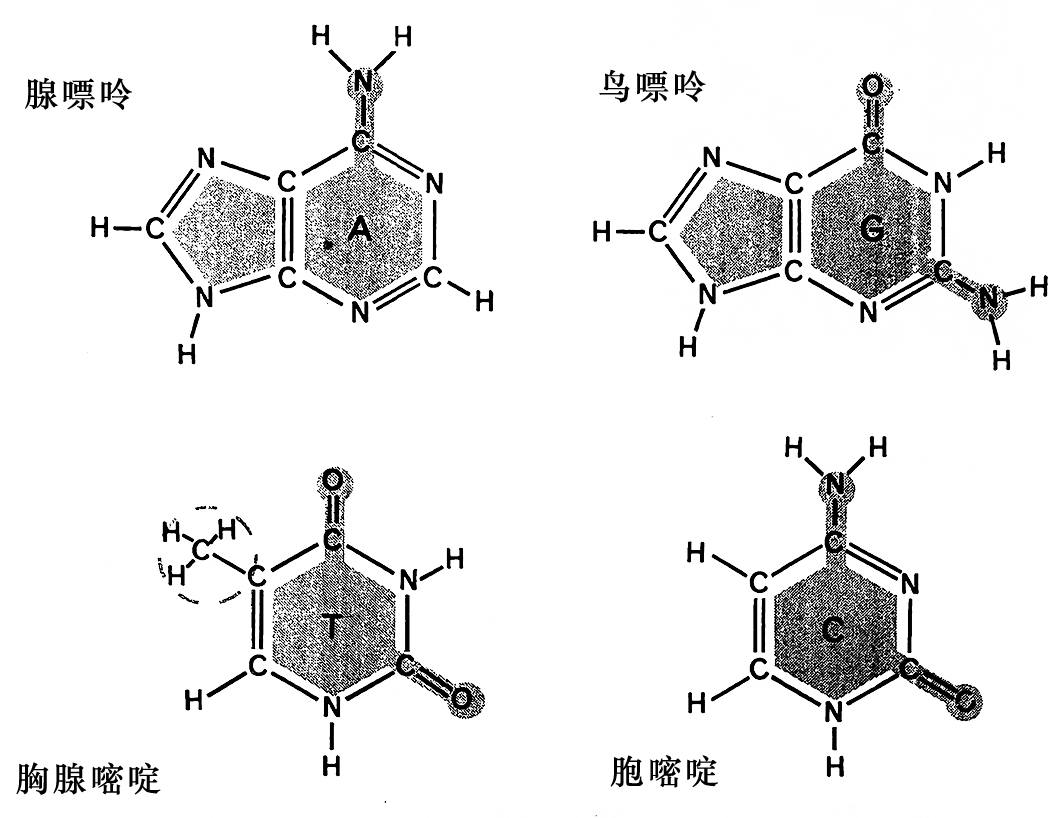
\includegraphics{img_091.png}
\caption[DNA的四种基。]
  {DNA的四种基:腺嘌呤,鸟嘌呤,胞嘧啶,胸腺嘧啶。[摘自哈瓦那尔特和海因斯[Hanawalt; Haynes],《生命的化学基础》[\bn{The Chemical Basis of Life}],旧金山:W. H. Freeman,1973年版,第142页。]}
\end{figure}

一个DNA串就这样由彼此串在一起的许多核苷酸组成,像一串珍珠一样。使一个核苷酸与其两边邻居相连的化学键很强,称作共价键,而“珍珠串”通常叫做DNA的共价脊柱。

\begin{figure}
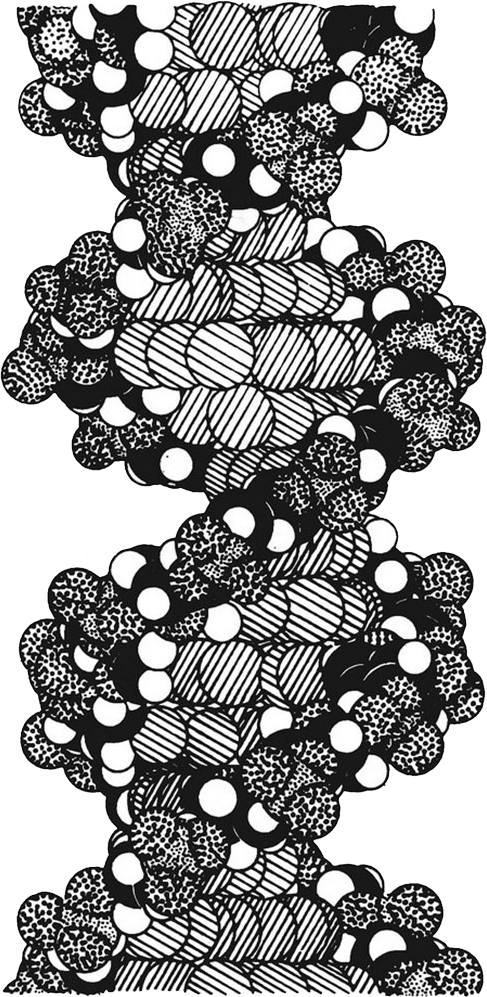
\includegraphics[height=.8\textheight]{img_092.png}
\caption[DNA的梯状结构。]
  {DNA结构象一架梯子。边上两条由脱氧核糖和磷酸盐的单元交替组成,横档以特殊方式配对——A配T,G配C——的基形成,基之间分别由两个或三个氧键相互连接。[摘自哈那瓦尔特和海因斯,《生命的化学基础》,第142页。]}
\end{figure}

DNA通常由一对串构成——就是说,由两条逐个配对的核苷酸串组成(见\fig{92})。站在两个串之间负责这种特殊类型的配对的是基。这个串中的每个基面对着另一个串中的补基,并拴住它。互补关系就像印符遗传学中一样:A与T配对,C与G配对,总是一个嘌呤配一个嘧啶。

与顺着脊柱方向的强共价键相比,串之间的键是相当弱的。它们不是共价键,而是氢键。氢键出现时,两个分子络合物以下面的方式相互结合:原先属于其中一个分子的某个氢原子,变得“弄不清”属于哪边了。它游移于两个络合体之间,不知加入哪一边好。由于双串型DNA的两个部分只靠氢键彼此相联,所以比较容易把它们分开,也比较容易结合。这一事实对细胞的工作至关重要。

DNA形成双串时,两个串彼此缠绕,像扭在一起的藤条(\fig{93})。每缠一圈恰好有十个核苷酸对,换句话说,每个核苷酸“扭”$36$度。单串型DNA就不是这种盘绕状,因为这是基对的产物。

\begin{figure}
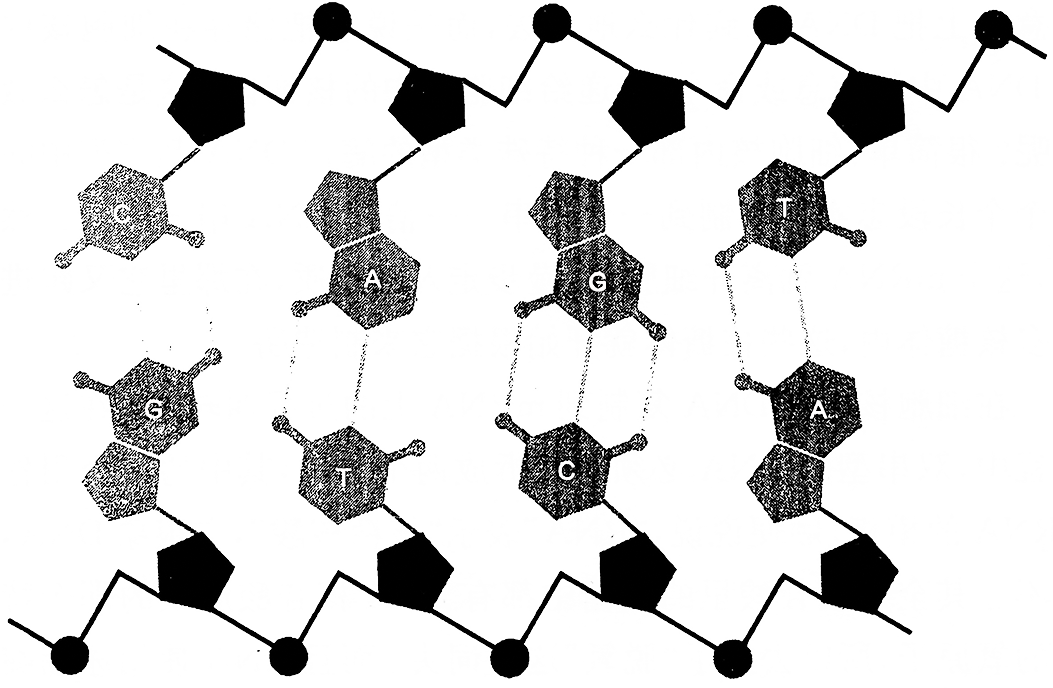
\includegraphics{img_093.png}
\caption[DNA的双螺旋分子模型。]
  {DNA的双螺旋分子模型。[摘自维农·英格莱姆[Vernon M. Ingraml,《生物合成》[\bn{Biosynthesis}],加利福尼亚州,Menlo Park: W. A. Benjamin,1972年版,第13页。]}
\end{figure}

\section{信使RNA与核糖体}

如上所述,在很多细胞里,DNA这个细胞君主住在隐蔽的“金銮殿”——细胞核——之内。但细胞中的大多数“活物”都在核外,即在细胞质中——那个相对于细胞核“图形”而言的“衬底”。特别是实际主宰着每个生命进程的酶,是在细胞质中由核糖体产生的,而且酶的大多数工作都在细胞质中进行。如同印符遗传学一样,全部酶的蓝图都储存在串里——即在DNA里,而DNA又藏在小小的细胞核之中。那么有关酶的结构的信息是怎样从细胞核里传给核糖体的呢?

这就该引入信使RNA——mRNA了。早先,mRNA曾被戏称为一种DNA“邮政快递”服务机构。这并不意味着mRNA在物理意义上把DNA带到什么地方去,而是说它把储存在细胞核内的DNA中的信息或命令,传递给细胞质中的核糖体。这是怎么做的呢?很简单:细胞核内部一种特殊类型的酶把DNA基序列中的一个个长段忠实地复制到一个新串——信使RNA串——上。然后,这个mRNA就离开细胞核,漫步走入细胞质,在那里它又跑进很多核糖体内,这些核糖体就开始根据它来制造酶。

在细胞核内把DNA复制到mRNA上的过程叫转录。在这一过程中,双串型的DNA必须暂时拆成两个单串,其中的一个用作mRNA的模板。顺便说说,“RNA”表示“核糖核酸”,它很像DNA,只不过其全部核苷酸里的核糖中都有DNA核苷酸所缺的那个特殊的氧原子,所以去掉了“脱氧”这个词头。而且RNA使用尿嘧啶这个基,而没有胸腺嘧啶,所以RNA串中的信息可以用“A”、“C”、“G”、“U”四个字母的任意序列来表示。从mRNA转录出DNA时,转录过程可以通过常用的基配对法来进行(不过这时不再有T了,而是U),所以,这种DNA模板与其mRNA伴侣看上去有点像是这样:
\begin{alignat*}{2}
\mathrm{DNA}:&\quad\dotsc\mathrm{CGTAAATCAAGTCA}\dotsc  &\quad&\text{(模板)}\\
\mathrm{mRNA}:&\quad\dotsc\mathrm{GCAUUUAGUUCAGU}\dotsc &     &\text{(“副本”)}
\end{alignat*}
RNA并不总与自己形成长的双串,尽管它能这样做。所以一般说来,它不是处于DNA的那种螺旋状态中,而是一个长长的、有时带点弯的串。

一个mRNA串一旦离开细胞核,就会遇到那些奇妙的亚细胞物质——“核糖体”。不过,在继续解释核糖体如何使用mRNA之前,我想对酶和蛋白质做些说明。酶属于分子生物学中所谓的蛋白质这样一个一般性范畴,而核糖体的工作是制造所有的蛋白质,并不只是制造酶。不是酶的那些蛋白质多是一些不活跃的家伙,例如,它们中有很多是结构分子,这意味着它们像是建筑物中的梁、柱等等:它们把细胞的各个部分连在一起。还有其他一些种类的蛋白质。不过就我们的目的而言,主要的蛋白质是酶,今后就不再特别区分了。

\section{氨基酸}

蛋白质由一系列氨基酸组成。氨基酸共有二十个品种,每一种都由三个字母来表示:
\begin{longtable}[c]{r!{——}l!{\qquad}r!{——}l}
ala & 丙氨酸 &
arg & 精氨酸\\
asn & 天门冬氨酰胺 &
asp & 天门冬氨酸\\
cys & 胱氨酸 &
gln & 谷酰胺\\
glu & 谷氨酸 &
gly & 甘氨酸\\
his & 组氨酸 &
ile & 异白氨酸\\
leu & 白氨酸 &
lys & 赖氨酸\\
mef & 蛋氨酸 &
phe & 苯基丙氨酸\\
pro & 脯氨酸 &
ser & 丝氨酸\\
thr & 苏氨酸 &
trp & 色氨酸\\
tyr & 酪氨酸 &
val & 缬氨酸
\end{longtable}
应当注意到这里与印符遗传学在数目上的轻微差别,在那里,我们只有十五种用以组成酶的氨基酸。氨基酸是大体上与核苷酸同样复杂的一个小分子,因而,建造蛋白质的砖块与建造核酸(DNA、RNA)的砖块差不多大。但是蛋白质是由短得多的序列组成的:在典型的情形,大约三百个氨基酸就组成一个完整的蛋白质,而一个DNA串却可以含有数十万乃至上百万个核苷酸。

\section{核糖体与录音机}

当一个mRNA串游离出来进入细胞质,然后遇到一个核糖体时,会发生一个极其复杂而又精彩的过程,我们称之为翻译。可以说,这个翻译过程就是一切生命的根本所在,其上罩着许多神秘的光环。不过,从本质上说,描述它并不难。我们先做一个形象化的比喻,然后再比较严格地加以说明。把mRNA设想成一长条录音磁带,而核糖体就像一台录音机。当磁带通过录音机的放音磁头时,信号就被“读出”并转变成音乐或其它声响。就这样,磁记号“翻译”成了音符。与此类似,当mRNA“磁带”通过核糖体的“放音磁头”时,产生出的音符是氨基酸,而作出的“乐曲”是蛋白质。所谓翻译也就是这些。\fig{96}表明了这一点。

\section{遗传密码}

\vspace{-\dp\strutbox}

\begin{lrbox}{\TEMPBOX}
\begin{minipage}{\dimexpr\linewidth/3\relax}
\small\medskip
\begingroup\centering\begin{tabular}{c}
CUA\quad GAU\\
Cu\hfill Ag\hfill Au
\end{tabular}\par\endgroup
\medskip\quotefont
一个典型的mRNA片段。先读成两个三元组(上面),然后读成三个二元组(下面):生物化学中的一个“三比二”的例子。
\end{minipage}
\end{lrbox}

\setlength\lwindowsep{\ccwd}
\setlength\rwindowsep{\lwindowsep}
\begin{window}[4,c,\usebox\TEMPBOX,{}]
可是,一个核糖体在读到一系列核苷酸时,怎么能生产出一系列氨基酸呢?经过很多人的努力,这个秘密在六十年代初被揭开了。答案的核心是遗传密码——从核苷酸的三元组到氨基酸的映射(见\fig{94})。这与印符遗传密码在精神上极为相似,除了这里是三个连续的基(或核苷酸)形成一个密码子,而在那里只要两个基就行了。因而,现在的表上必定要有$4\times4\times4$(即$64$)个不同条目,而不只是十六个。核糖体一次从RNA串上切下三个核苷酸——也就是说,一次切一个密码子——而且,它每这样做一次,就把一个单独的新氨基酸加到了正在生产的蛋白质上。于是,蛋白质就一个氨基酸接一个氨基酸地从核糖体中制造出来了。
\end{window}

\begin{figure}
%\includegraphics{img_094.png}
\def\OLW{\heavyrulewidth}
\def\MLW{\lightrulewidth}
%\tabulinesep=.5ex\relax
\begin{tabu} to .8\linewidth{>{\Large}X[.75,c]*4{|X[c]}|X[.5,c]}
\tabucline[\OLW]-
\rowfont{\large}
 & U & C & A & G & \\ \tabucline[\MLW]-
\multirow{4}{*}{U}
  & phe & ser & tyr & cys & U \\
  & phe & ser & tyr & cys & C \\
  & leu & ser & 标点  & 标点  & A \\
  & leu & ser & 标点 & trp & G \\ \tabucline-
\multirow{4}{*}{C}
  & leu & pro & his & arg & U \\
  & leu & pro & his & arg & C \\
  & leu & pro & gin & arg & A \\
  & leu & pro & gin & arg & G \\ \tabucline-
\multirow{4}{*}{A}
  & ile & thr & asn & ser & U \\
  & ile & thr & asn & ser & C \\
  & ile & thr & lys & arg & A \\
  & met & thr & lys & arg & G \\ \tabucline-
\multirow{4}{*}{G}
  & val & ala & asp & gly & U \\
  & val & ala & asp & gly & C \\
  & val & ala & glu & gly & A \\
  & val & ala & glu & gly & G \\
\tabucline[\OLW]-
\end{tabu}
\caption[遗传密码。]
  {遗传密码。信使RNA串中的每个三元组就这样为二十种氮基酸(及一个标点符号)编码。}
\end{figure}

\section{三级结构}

然而,随着一个蛋白质从核糖体中走出来,它不仅会越来越长,而且会逐渐地折叠成一个奇特的三维形状,很像是那种滑稽的蛇形焰火,在点亮时一面伸长,一面卷曲。这种形状称作蛋白质的三级结构(\fig{95}),而原先的氨基酸序列叫做蛋白质的一级结构。这个三级结构暗含在一级结构之中,这正和印符遗传学的情形一样。

\begin{figure}
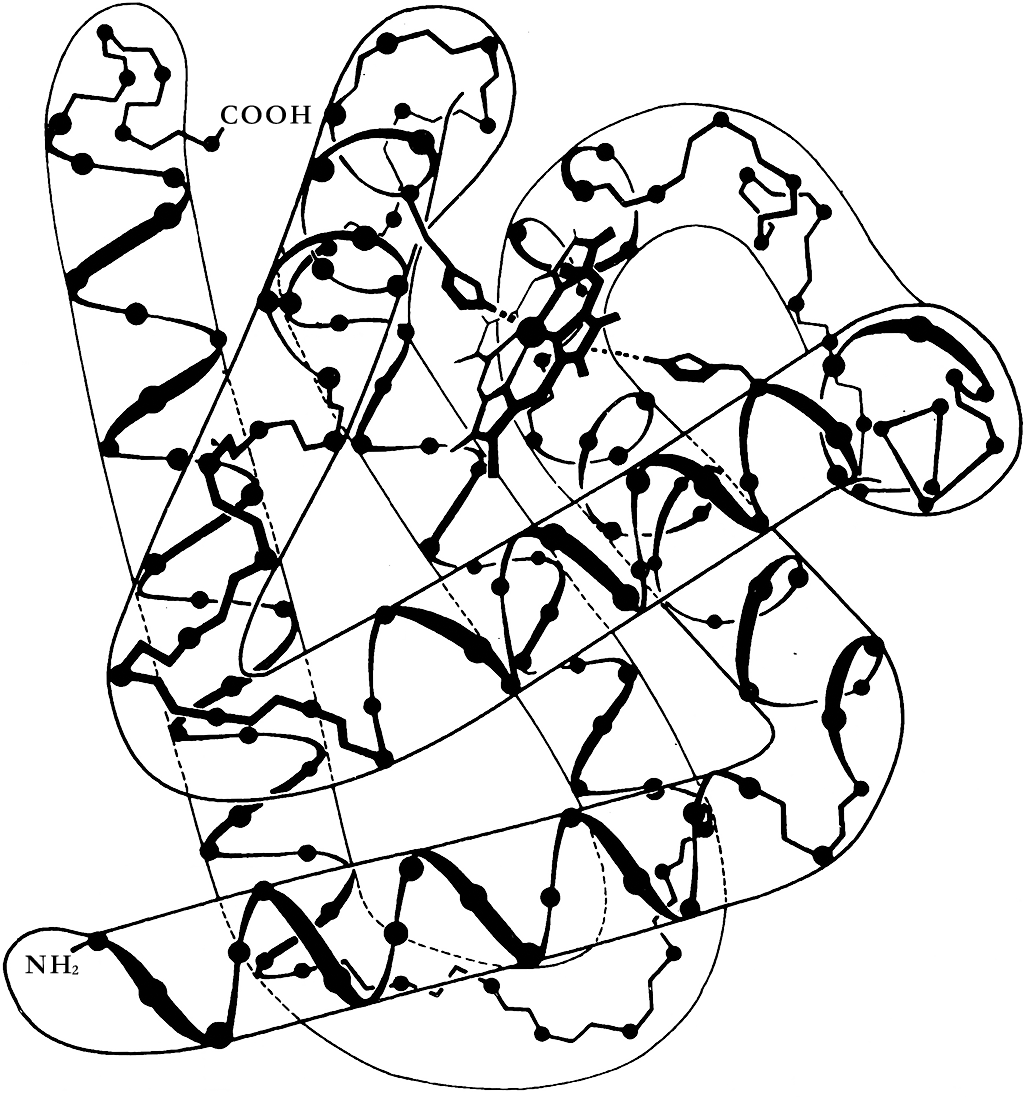
\includegraphics{img_095.png}
\caption[肌红蛋白的二级和三级结构。]
  {从一些高分辨率的X光资料推断出的肌红蛋白的结构。大尺寸的“扭曲管道”形状是三级结构,内部的细螺旋——“阿尔法螺旋”——是二级结构。[选自莱宁格尔,《生物化学》。]}
\end{figure}

可是,如果你只知道一级结构,那么导出三级结构的方法可就远比印符遗传学要复杂了。事实上,搞清某些规则,以便只要知道了蛋白质的一级结构就能指出其三级结构,乃是当代分子生物学中悬而未决的问题之一。

\section{蛋白质功能的简化论解释}

印符遗传学和真正遗传学之间的另一个差别——这可能是所有差别中最重要的一个——是:在印符遗传学中,组成酶的每个氨基酸都负责某个具体的“作用片断”;而在实际的酶中,单个的氨基酸不能充当这种明确的角色。确定酶的作用方式的,是作为一个整体的三级结构。不能说“这个氨基酸的存在就意味着如此这般的一个操作得以执行”这类的话。换言之,在实际遗传学中,一个单独的氨基酸对酶的整个功能的贡献不是“上下文无关”的。不过这一事实无论如何都不能当作反简化论者的武器以得出“整体(的酶)不能解释为其各部分之和”的结论。这种结论还完全没有得到验证。得到验证的东西是排除了下面这个简单的断言:“每个氨基酸都用一种不依赖其它氨基酸的存在的方式对总体发生作用”。换句话说,酶的功能不能看成是由各个部分的上下文无关的功能建立起来的,而必须考虑各部分之间的相互作用。原则上,仍有可能写出一个计算机程序把蛋白质的一级结构作为输入,然后先确定其三级结构,再确定酶的功能。这将是对蛋白质工作的一个彻底的简化论解释,但要确定各部分的“总和”得需要一个高度复杂的算法。在给出酶的一级的、乃至三级的结构之后,如何阐明酶的功能是现代分子生物学的又一个大问题。

也许,整个酶的功能最终仍可以看成是按照一种上下文无关的方法,从各个部分的功能上建立起来的,不过这里得把这些部分看成是单个的粒子,诸如电子、质子之类,而不是看成像氨基酸那样的“大块头”。这正是“简化主义者的窘境”:为了用上下文无关的总和这类概念来解释每一件事情,就必须降到物理的层次上,可是此时粒子的数目会如此之大,以至于只能说出理论上“大概”如何之类的话。所以我们只好满足于一个上下文有关的总和。它又有两个缺点,第一,总和的各个部分是相当大的单元,其性状就只能在高层次上描述,因而并不确定。第二,“总和”这个词意味着:每个部分都分担一个简单的功能,而整体的功能正好是这些个别功能的一个上下文无关的总和。当我们在给定一个酶的各个氨基酸后要解释整个酶的功能时,却正好做不到这一点。但不论是吉是凶,这是解释复杂系统时总要发生的一般现象。为了对各部分之间如何相互作用有一个既直观又易于处理的理解——简言之,为了能继续下去——我们时常不得不牺牲掉依靠微观的及上下文无关的画面所能得到的精确性。这纯粹是因为它不易处理。但此时不必失去信心,以致怀疑这样一个解释在原则上是否存在。

\section{转移RNA与核糖体}

现在我们回到核糖体、RNA和蛋白质。前面已经说过,蛋白质是核糖体根据DNA的信使RNA从DNA的“金銮殿”带来的蓝图生产的。这似乎蕴涵着核糖体可以把密码子的语言翻译成氨基酸的语言,而这又等于说核糖体“懂得”密码。然而,全部信息恰恰并不在核糖体内。它是怎么做到的呢?遗传密码贮存在哪里呢?令人惊异的事实是:遗传密码就在——还能在哪儿呢?——DNA自身之内。这当然要作些解释。

我们把总体的解释丢开一会儿,先给出一个部分的解释。在任何给定的时刻,细胞质周围都四散漂浮着大量的四叶草形分子,在它们的一个叶片上,松松地拴着(即靠氢键相连)一个氨基酸,而在对面的叶片上有一个称为反密码子的核苷酸三元组。就我们的目的而言,另外两个叶片无关紧要。下面说明核糖体在制造蛋白质时如何使用这些“草”。当一个新的mRNA密码子进入核糖体的“放音磁头”的位置时,核糖体就伸手到细胞质中抓住一片其反密码子恰与该mRNA密码子互补的草,然后把这片草拽到这样一个位置上:能揭下叶子上的氨基酸,用一个共价键把它粘到正在生成的蛋白质上(顺便说一句,一个氨基酸在蛋白质中与其邻居之间的键是一种很强的共价键,称为“肽键”。因此,蛋白质有时也叫“多肽”)。当然,“草”上带有合适的氨基酸并不是偶然的,因为它们全是根据来自“金銮殿”的严格指令生产出来的。

\begin{figure}
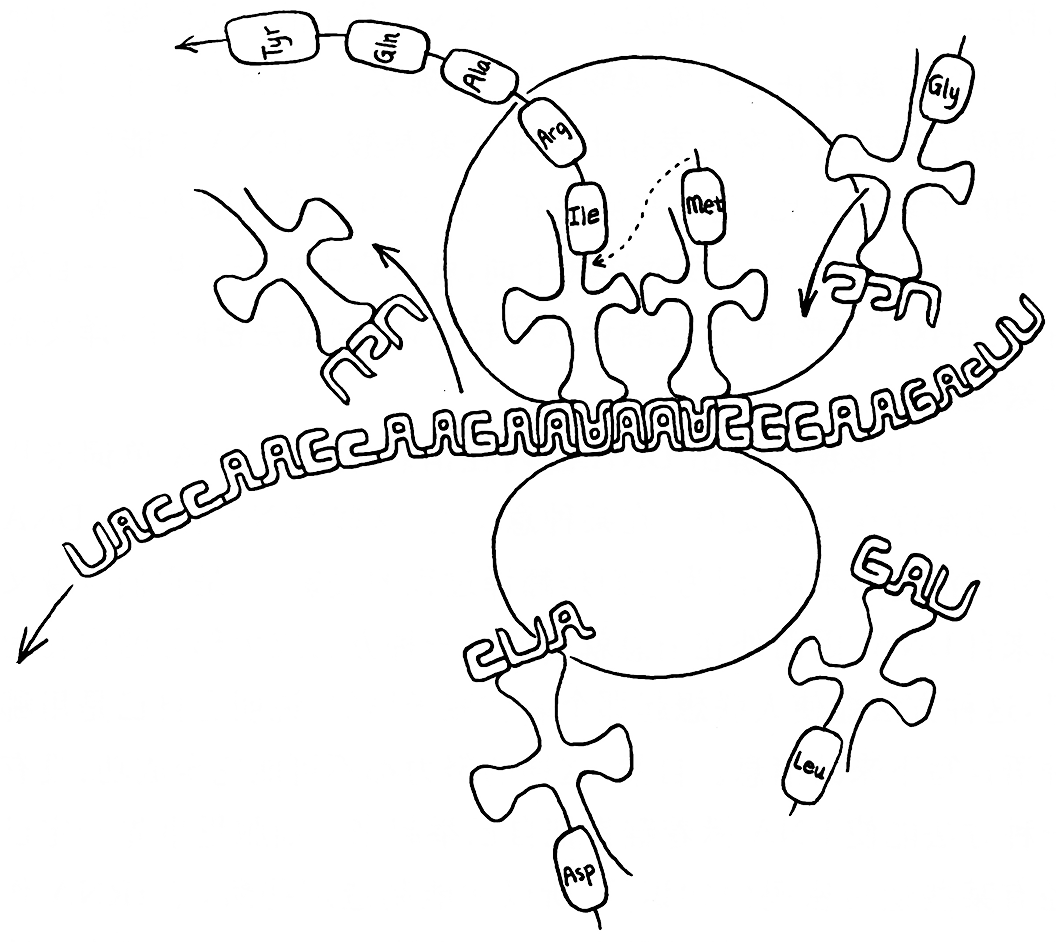
\includegraphics{img_096.png}
\caption[一段mRNA通过核糖体。]
  {一段mRNA通过核糖体。漂浮在附近的是些tRNA分子,它们带有能被核糖体抓来并加进正在生成的蛋白质中的氨基酸。遗传密码作为一个整体包含在tRNA分子内。要注意,基对(A-U,C-G)在图中由卡在一起的字型表示。[斯科特·凯姆绘]}
\end{figure}

这种草的真正名字叫转移RNA(tRNA)。tRNA分子相当小——大约相当于一个很小的蛋白质分子的尺寸——含有大约八十个核苷酸组成的一个链。与mRNA类似,tRNA分子由主要的细胞模板DNA转录出来。可是,与含有数千个核苷酸形成的大长链的庞大mRNA分子相比,tRNA是个侏儒。此外,tRNA在这方面更像蛋白质(而不像mRNA串):它们都有确定的、良定义的三级结构——由其一级结构确定。一个tRNA分子的三级结构恰好允许一个氨基酸拴在它的氨基酸位置上。确实,它就是对面叶片上的反密码子根据遗传密码表指出的那个氨基酸。tRNA功能的一个生动的形象化类比,是一些漂浮在一位同声翻译周围的云雾之中的单词卡片,只要他需要翻译某个词,就从空中抓来一片——百发百中!在这种情形中,这位翻译就是核糖体,词就是密码子,译文就是氨基酸。

为了让核糖体解出DNA的内在消息,这些tRNA单词卡片就必须漂浮在细胞质中。在某种意义上,这些tRNA包含了DNA的外在消息的本质,因为它们是翻译过程的关键。但是它们自身又都来自DNA。因而外在消息就要通过一种方法成为部分的内在消息,这种方法能使人联想起那个装在瓶子里的、说明它自己是用哪种语言写下来的消息。自然,这样的努力都不可能完全成功:没有一种方法能使DNA揪着鞋带把自己举起来。细胞里事先一定已经有某些遗传密码的知识了,所以才能制造那些酶,把tRNA作为DNA的主要副本给转录出来。而这种知识又储存在早先制造好的那些tRNA分子之内。这种完全排除对外在消息需要的努力就像艾舍尔的那条龙,在困住它的那个二维世界的环境中,它竭尽全力想要成为三维的,它似乎做了很多——不过当然决不会成功,尽管它给出了三维性的一个很好的模拟。

\section{标点和阅读框架}

核糖体怎么会知道什么时候一个蛋白质就制作好了呢?和印符遗传学一样,mRNA中也有一个记号,指示出一个蛋白质的结束或开始。事实上,有三个特殊的密码子——UAA、UAG、UGA——都起标点符号的作用,而不是给氨基酸编码。当这样的一个三元组一下一下地滑入核糖体的“放音磁头”时,核糖体就放走正在构造的那个蛋白质,然后开始构造一个新的蛋白质。

最近,已经揭示了已知的最小病毒$\varphi\mathrm{X}174$的全部基因组。一项极为意外的发现正在完成之中:它的$9$个基因中,有一些是部分重叠的——也就是说,两个不同的蛋白质由同一个DNA段编码!甚至有一个基因整个地包含在另一个里面!之所以如此,是因为两个基因的阅读框架彼此恰好错开一个单元。按这种方式压缩信息所导致的稠密性是难以置信的。当然,这正是《音程增值的卡农》里藏在阿基里斯的福气小甜饼中那奇妙的“$4/17$俳句”后面的灵感。

\section{概括}

于是,简而言之,我们眼前是这样一幅画面:从DNA御座出发,DNA把信使RNA的一些长串送到细胞质中的核糖体上;而核糖体利用盘旋在自己周围的那些tRNA“单词卡片”,根据mRNA中含有的蓝图,一个氨基酸接一个氨基酸地、高效率地构造蛋白质。DNA仅指示了蛋白质的一级结构。但这足够了,因为当蛋白质从核糖体中出来时,它们便“魔术般地”折叠成复杂的形态,从而有能力像一台大功率的化学机器一样行动。

\section{蛋白质与音乐中的多层结构和意义}

我们已经把核糖体的形象比作录音机,mRNA比作磁带,而蛋白质则是音乐。这看上去像是信手掂来,然而它们之间却有一些精彩的平行之处。音乐不仅仅是线性的音符序列。我们的心智是在比这高得多的层次上来理解乐曲的。我们把音符组块化成为乐句,若干乐句构成旋律,一些旋律形成乐章,几个乐章组成全曲。类似地,蛋白质只有在作为组块化单元起作用时才有意义。尽管一级结构已经携带着制造三级结构所需要的全部信息,但仍然“嫌少”,因为只有在物理上实际造出这个三级结构来,才能理解其潜力。

顺带提一句,我们只说到一级结构和三级结构,读者可能会奇怪:二级结构哪去了?其实是有的,就连四级结构也有。蛋白质的折叠现象不止存在于一个层次上。具体讲,在氨基酸链的某些地方,有形成一种螺旋的趋势,这叫阿尔法螺旋(别与DNA双螺旋搞混)。蛋白质的这种螺旋形扭曲处在比其三级结构低的层次上。这一层结构可以在\fig{95}中看到。四级结构可以比拟成由独立乐章组成的整个乐曲大厦,因为它牵涉到把已经绽开三级鲜花的若干不同的多肽组合成一个更大的结构。这些独立的链之间通常由氢键相连,而不是靠共价键。当然,这正像一个由若干乐章组成的乐曲,其各章之间的联系远不如章内的联系紧密,但仍能形成一个“有机”的整体。

一级结构、二级结构、三级结构和四级结构,这四个层次还可以比作《前奏曲,蚂蚁赋格》中的“无之图”(\fig{60})的四个层次。总的结构——由两横一撇及一个竖弯钩组成一个“无”字——是它的四级结构;那两横及那一撇一竖弯钩本身是三级结构,分别由“整体论”和“简化论”组成;而三级结构的“整体论”与“简化论”其笔划分别由二级结构的“简化论”和“整体论”组成,最后,一级结构则是一遍又一遍地重复“无”字。

\section{多核糖体与二排卡农}

我们再来看看把磁带翻译成音乐的录音机,与把mRNA翻译成蛋白质的核糖体两者之间的另一个优美的平行关系。设想有许多磁带录音机一字排开,间隔相等。我们可以把这个阵势叫做“多录音机”。再设想同一条磁带陆续通过各个录音机的放音磁头,如果磁带上录有一个完整的长旋律,那么输出自然是一个多部轮唱,各声部之间的延迟由磁带从一台录音机起到下一台录音机所用的时间来确定。在细胞中,确实也存在这种“分子卡农”,那里,很多核糖体一字排开,形成所谓多核糖体。它们全都“使用”同一个mRNA串,错开一定时间,生产同样的蛋白质(见\fig{97})。

\begin{figure}
\fcapside[\FBwidth]{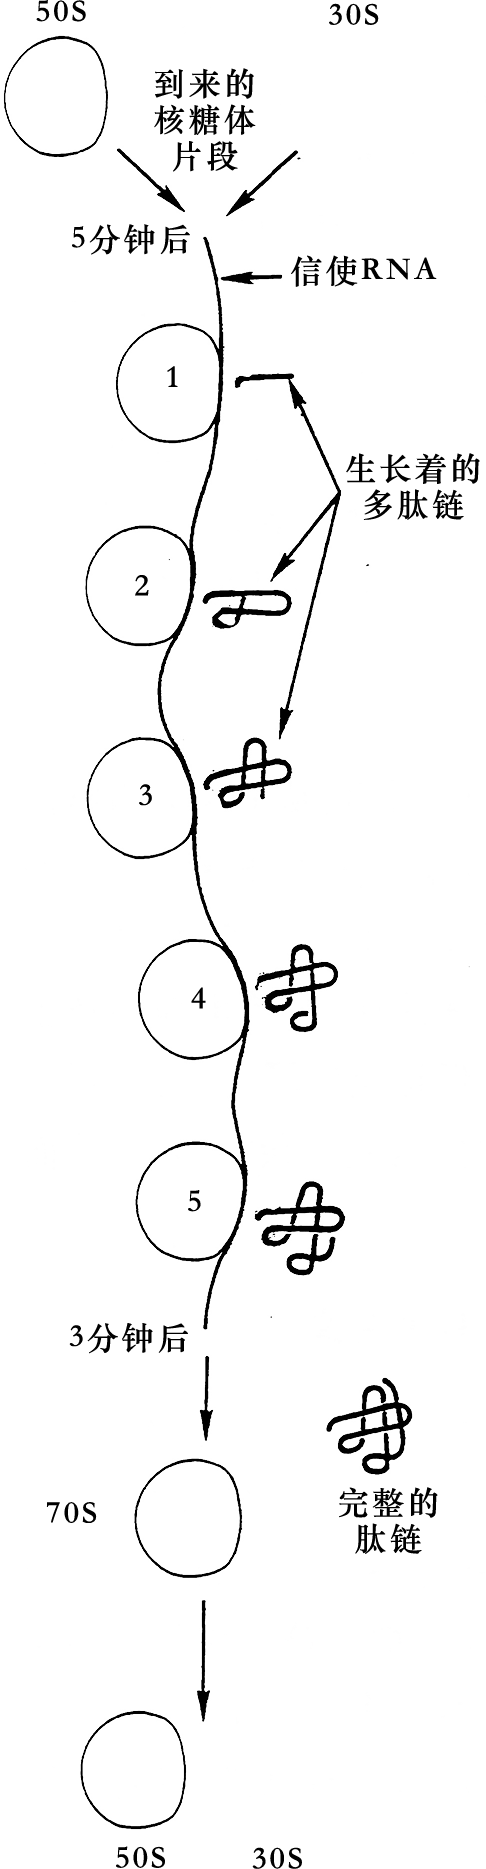
\includegraphics[height=\textheight]{img_097.png}}{%
\caption[多核糖体。]
  {多核糖体。同一个mRNA串通过一个接一个的核糖体,就好象磁带依次通过若干台录音机。其结果是一批处于不同程度的正在生成的蛋白质:类似于相互错开的若干录音机所生成的音乐卡农。[选自莱宁格尔,《生物化学》。]}}
\end{figure}

不仅如此,大自然做得还要好些。我们还记得,mRNA是通过转录DNA而制成的,负责这个过程的酶叫RNA聚合酶。常有这样的事发生:一系列RNA聚合酶会并排工作在同一个DNA串上,结果就造出很多彼此分离(但却相同)的mRNA串,每一串都相对上一串延迟一点时间,这正是DNA从一个RNA聚合酶移到下一个聚合酶所需要的时间。同时,在并排出现的每一个mRNA上,又可以有若干不同的核糖体在工作。这样,就达到了一个双层的或二排的“分子卡农”(\fig{98})。在音乐中的对应形象是一个十分荒唐但却很有意思的情景:若干名誊写员同时工作,每个人都把一份原稿从长笛手无法演奏的谱表抄成一个他们能演奏的谱表。每个誊写员抄完一页原稿,就把原稿传给下个人,然后自己再抄新的一页。与此同时,根据出自每个誊写员笔下的抄件,有一组长笛在吹奏这个旋律,每个长笛手相对于其他吹奏同一张曲谱的人又有所延迟。也许这个极度夸张的形象能使你对你身体中每分每秒都在进行着的过程的复杂性的某些方面有所想象。

\begin{figure}
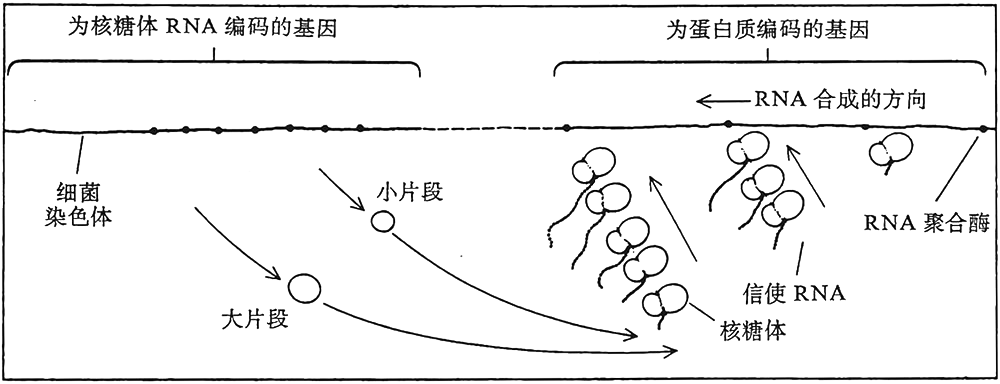
\includegraphics{img_098.png}
\caption[二排的分子卡农。]
  {这里是一个更为复杂的图示,不只一个而是有若干个mRNA串,它们全都转录自同一个DNA串,并受到多核糖体作用,其结果是一个二排的分子卡农。[选自哈那瓦尔特和海因斯,《生命的化学基础》,第271页。]}
\end{figure}

\section{谁生谁——核糖体与蛋白质}

我们一直在谈论那些称为核糖体的惊人活物,可它们自己又是怎么构成的、如何制造的呢?核糖体由两种东西构成:\pnum{1}各类蛋白质,\pnum{2}另一种RNA,叫做核糖体RNA(rRNA)。于是,为了造出核糖体,得有某些种类的蛋白质,还得有rRNA。自然,要有蛋白质就得有核糖体来制造它。那么,你怎么应付这个恶性循环呢?先有谁——核糖体还是蛋白质?谁制造谁?当然不会有答案,因为往前追溯总是会遇到当前对象的同类——就像先有鸡还是先有蛋的问题一样——直到一切都消失在时间的地平线上为止。无论何时,核糖体总是由两块东西制成,一大一小,每一块中都含有一个rRNA和几个蛋白质。核糖体差不多和大的蛋白质一样大小。它们远远小于作为它们的输入并且它们要顺着移动的mRNA串。

\section{蛋白质的功能}

我们已经谈过一些蛋白质的结构,尤其是酶的结构,但我们还没有实际讲述它们在细胞内执行什么任务,以及如何去做。全部的酶都是催化剂,这意味着,在某种意义上,它不过是有选择地加速细胞中的一些化学过程,而不是使那些没有它们就不能发生的事情发生。每种酶都使千万条潜在通道中的一条特定通道得以实现。因此,在选定要引入哪一种酶的同时,你也就选定了将要发生的事情和将不发生的事情——尽管从理论上说,任何细胞过程不靠催化剂帮助而自动发生的概率都不是零。

酶怎样在细胞里的分子上起作用呢?如已经讲过的那样,酶是折起的多肽链,每个酶中都有一个裂缝或口袋或某种别的清晰定义的外观特性,酶在那里拴住某个其它种类的分子。这个地点叫活性部位,拴在那里的分子叫基质。酶可以有不止一个活性部位和不只一个基质。像印符遗传学一样,酶对于它们所要发挥作用的部位实在是很挑剔的。活性部位通常都很“挑食”:只许一种分子拴在上面。尽管如此,有时也会遇上“李鬼”——一些其它分子,它们也能适应这个作用点并赘在上面,哄骗这个酶,从而事实上使酶起不了作用。

一旦把酶与其基质拴在一起,就会发生某种电荷不平衡状态,随后,电荷——以电子或质子的形式——就围绕着拴住的分子流动并重新排布自己。达到平衡时,基质可能已经发生了意义深刻的化学变化。例如:可能已经发生了一个“焊接”过程,把一些标准的小分子连成核苷酸、氨基酸或其它的普通细胞分子;一个DNA串可能已在一个特殊的部位“豁开”;一个分子的某一部分可能已被割掉;等等,等等。事实上,生物酶对分子所起的作用十分类似于印符酶所执行的印符操作。只不过大多数酶基本上都只执行单项任务,而不是执行一系列任务。印符酶和生物酶之间还有一个显著的区别,那就是:印符酶只作用在串上,而生物酶则可以作用在DNA、RNA、其它蛋白质、核糖体以及细胞膜之上——简言之,作用于细胞里的每一样东西。换句话说,酶是在细胞内使各种事件得以发生的通用机器。有各种各样的酶,有的能把东西粘在一起,有的又把它们分开,有的修改它们,有的激活它们,有的安定它们,有的复制它们,有的恢复它们,有的毁坏它们……

细胞内某些极为复杂的过程是“多级瀑布”形的,在那里面,某种类型的单个分子导致某种酶的生产过程;生产过程开始后,从“组装线”中制出的酶又开辟一条新的化学途经使第二种酶开始生产。这种事情可以持续三四层,每一种新生产出的酶又引起另一类型的生产过程。最后,生产出一大批最终型号的酶的副本,然后所有的副本就脱离出来,去执行它们各自的任务,也许是去除掉某个“异端”DNA,或协助制作细胞所“渴望”的某种氨基酸,或是别的什么事情。

\section{需要有一个足够强有力的支撑系统}

我们来说说印符遗传学所揭示的大自然对“什么样的DNA串能指挥自己的复制?”这个谜题的解答。当然,并非每个DNA串生来都是自复制。关键在于:任何一个想要指挥自己的复制工作的串,都必须含有一些命令,以便能恰好调集那些能够执行这一任务的酶。指望一个DNA串孤家寡人就能成为自复制,这是枉费心机。因为,要把那些潜在的蛋白质从DNA中拽出来,不仅得有核糖体,而且还得有RNA催化酶。后者要用来制造输送给核糖体的mRNA。所以我们必须从假定有一种刚好强到允许转录过程和翻译过程得以进行的“极小支撑系统”开始。于是,这个极小支撑系统就得包括:\pnum{1}某些保证mRNA能从DNA制造出来的蛋白质——例如RNA聚合酶,\pnum{2}某些核糖体。

\section{DNA如何自复制}

“足够强有力的支撑系统”和“足够强有力的形式系统”两种说法听起来很有些相似,这无论如何不能算是巧合。一个是产生自复制的前提,一个是产生自指的前提。其实,从本质上讲,这只是一种现象在两个不同的外观下出现,而我们马上就要把它们明显地对应起来。不过,做这件事情以前,我们先得说清楚一个DNA串怎么能成为自复制。

DNA必定含有一组蛋白质的密码,而这组蛋白质就将复制这个DNA。有一种十分有效而精致的办法能复制一个由互补的两个串组成的双串DNA。这包括两步:
\begin{enumerate}
\item 把两个串彼此分开,
\item 给刚刚得到的两个新的单串各“配”上一个新串。
\end{enumerate}
这个过程能造出两个新的DNA串,每一个都与原先的双串等同。如果我们的解决办法是建立在这个想法上的,那就必定要涉及一组在DNA中有自己的密码、并将要执行这两个步骤的蛋白质。

据信,在细胞内这两个步骤是通过一种协调的方式一起进行的,而且需要三种主要的酶:DNA核酸内切酶,DNA催化酶和DNA连接酶。第一种是个“拉开酶”:它把原有的两个串剥开一小段距离,然后停止。这之后,另外两种酶登场。催化酶基本上是一种完成“复制并移动”操作的酶:它切下DNA的一个短短的单串,以一种会使人联想起印符遗传学中的复制状态的方式用补基来复制它们。为了复制,它要利用在细胞质中四处漂浮的一些原料——尤其是核苷酸。由于这个过程是阵发性的,每次都剥开一些东西,复制一些东西,所以就产生了一些小缝隙,而DNA连接酶就是堵缝的东西。这个过程一遍又一遍地重复。这部精密的三酶机就以一种小心翼翼的方式一路沿着DNA分子运行着,直到整个东西都被剥开,同时也被复制,最后有了两个副本为止。

\section{DNA的自复制方法与㧟摁相比较}

应该注意,在酶对DNA串的作用过程中,全然没有用到信息储存在DNA之中这一事实。酶只是在执行调拨符号的职能,就像"WJU"系统中的推理规则一样。这三种酶在某一时刻就在实际复制作为他们自身的密码的那些基因,但它们对此却无动于衷。对它们来说,DNA只是一块既无意义也无趣味的模板。

把这与蒯恩句子那种描述如何构造自己的副本的方法作个比较是颇为有趣的。在那里,也有一种“双串”——同一信息的两个副本,其中一个起指令作用,另一个起模板作用。在DNA中,过程有一点类似,因为三种酶(DNA核酸内切酶、DNA催化酶、DNA连接酶)只在其中的一个串中被编码,这个串就起着程序的作用,而另一个串只是块模板。这个平行还不完美,因为在执行一个复制动作时,两个串都作模板使用,而不只是一个串。即便如此,这个类比也是具有高度启发性的。对这种使用与谈论的二重性,有一个生物化学的类比:当DNA被看作只是一系列有待复制的化学物质时,就相当于谈论印刷符号;而当DNA指示该执行哪些操作时,就相当于使用印刷符号。

\section{DNA的意义层次}

从一个DNA串里可以读出好几个不同层次的意义,这要看你把DNA划成多大的块,以及你使用的解码器有多强。在最低的层次上,每一个DNA串给一个等效的RNA串编码——作为转录的编码过程。如果将DNA组块而形成三元组,那么,利用“遗传解码器”就能把DNA读成一系列氨基酸。这是(在转录之上的)一个翻译。在下一个自然的层次上,DNA又可读成一组蛋白质的代码。这个把蛋白质从基因里拽出来的物理过程叫做基因表示。目前,这是我们所了解的DNA意义的最高层次了。

然而,肯定有更高层次的意义,它们更难觉察。例如,有种种理由使人们相信(比如说人的)DNA含有个人特征(如鼻子的形状、音乐天份、反应速度等等)方面的密码。我们能不能在原则上学会直接从一个DNA串读出这些信息,而不必经历实际的物理渐成过程(从遗传型到表现型的物理显示)呢?大概是可以的。因为在理论上我们可以拥有一个强得难以置信的计算机程序来模拟整个的过程,包括每个细胞、细胞中的每种蛋白质、以及DNA复制时所涉及的每个细微末节,等等,一直做到底。这样一个伪渐成程序就是表现型的一个高层次描述。

另外还有一种(极其微弱的)可能:我们毋需去同构模拟渐成过程,而是通过找到某种较为简单的解码器,直接从遗传型读出表现型来。这可以叫做“捷径伪渐成过程”。捷径也好,非捷径也好,伪渐成过程目前当然还远未达到——尽管有个惹人注目的例外:对于猫科的一个种——家猫[Felis-catus],深入的探索已经揭示出,确有可能直接从遗传型读出表现型来。直接观察一下家猫的DNA中下述典型节段,可能就会更好地体会这个值得注意的事实:\note{制作者注:“猫”在英语里是“CAT”。}
\begin{center}
\ldots CATCATCATCATCATCATCATCATCATCAT\ldots
\end{center}
下面列出了各个层次上DNA读出方式的一览表,以及不同的译码层次的名称。DNA能被读成这样的序列:
\begin{enumerate}
\item 基(核苷酸)\cdotfill 转录
\item 氨基酸\cdotfill 翻译

\item \indent
  \tikz[remember picture,inner sep=0pt,baseline=(N1.base)]
    \node(N1){蛋白质(一级结构)};\hfill
  \tikz[remember picture]\coordinate(L);%
\nopagebreak
\item \indent
  \tikz[remember picture,inner sep=0pt,baseline=(N2.base)]
    \node(N2){蛋白质(三级结构)};%
  \begin{tikzpicture}[remember picture, overlay,inner sep=0pt]
    \draw[decorate, decoration={brace,amplitude=2mm,raise=2mm}]
      (N1.north east) -- (N1.north east|-N2.south east)
        coordinate[midway,right=5mm](N12);
    \path
      (N12-|L) coordinate (NL12)
      let \p1 = (N12), \p2 = (NL12)
      in node[text width=\x2-\x1,left] {\cdotfill 基因表示};
  \end{tikzpicture}

\item 蛋白质束\cdotfill 高层基因表示

\item \indent
  \tikz[remember picture,inner sep=0pt,baseline=(N1.base)]
    \node(N1){???};\hfill
  \tikz[remember picture]\coordinate(L);%
\nopagebreak
\item[{\tikz[remember picture]\coordinate(R);\hphantom{)}}]\indent
\nopagebreak
\item[($N-1$)]\indent
  \tikz[remember picture,inner sep=0pt,baseline=(N2.base)]
    \node(N2){???};%
  \begin{tikzpicture}[remember picture, overlay,inner sep=0pt]
    \draw[decorate, decoration={brace,amplitude=2mm,raise=2mm}]
      (N1.north east) -- (N1.north east|-N2.south east)
        coordinate[midway,right=5mm](N12);
    \path
      ($(N1)!.5!(N2)$) node {$\vdots$}
      -| (R) node[midway,left] {$\vdots$}
      (N12-|L) coordinate (NL12)
      let \p1 = (N12), \p2 = (NL12)
      in node[text width=\x2-\x1,left] {\cdotfill DNA意义的未知层次};
  \end{tikzpicture}

\item[($N$)] 物理、精神和心理的品质 \cdotfill 伪渐成过程
\end{enumerate}

\section{中心法则映射}

有了这个背景,我们就可以在克里克的“分子生物学中心法则”(称做\emph{法则I},这是一切细胞过程的基础)和我富有诗意的发明——“数理逻辑中心法则”(称作\emph{法则II},是哥德尔定理的基础)——之间做一个精细的比较。\fig{99}和表~\ref{tab:central-dogmap} 显示了其间的映射,这个图和表一起构成了“中心法则映射”。

\begin{table}
\caption{中心法则映射。}\label{tab:central-dogmap}
\begin{tabu}[c]{@{}X[r]cX[l]@{}}
\toprule
\emph{法则I}(分子生物学) & & \emph{法则II}(数理逻辑)\\
\midrule
DNA串 & $\iff$ & TNT符号串\\
mRNA串 & $\iff$ & N的陈述\\
蛋白质 & $\iff$ & 元TNT的陈述\\
作用在蛋白质上的蛋白质 & $\iff$ & 关于元TNT的陈述的陈述\\
作用在作用在蛋白质上的\par 蛋白质上的蛋白质 & $\iff$ & 关于关于元TNT陈述的\par 陈述的陈述\strut\\
转录($\text{DNA}\Rightarrow\text{RNA}$) & $\iff$ & 解释($\TNT\Rightarrow\text{N}$)\\
翻译($\text{RNA}\Rightarrow\text{蛋白质}$) & $\iff$ & 算术化($\text{N}\Rightarrow\text{元TNT}$)\\
克里克 & $\iff$ & 哥德尔\\
遗传密码(任意约定) & $\iff$ & 哥德尔编码(任意约定)\\
密码子(基因的三元组) & $\iff$ & 密码子(数码的三元组)\\
氨基酸 & $\iff$ & 元TNT中引用的TNT符号\\
自复制 & $\iff$ & 自指\\
使自复制得以发生的\par 充分强的细胞系统 & $\iff$ & 使自指得以发生的\par 充分强的算术形式系统\strut\\
\bottomrule
\end{tabu}
\end{table}

\begin{figure}
%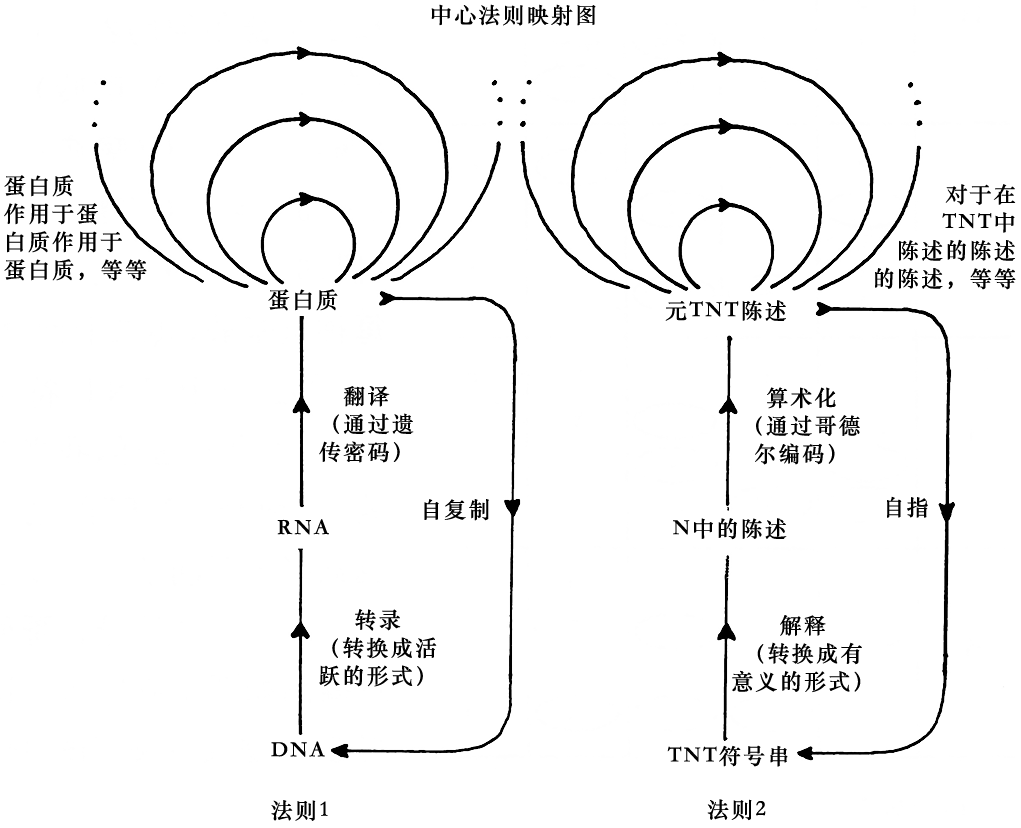
\includegraphics{img_099.png}
\begin{tikzpicture}[arrow decoration]
\path[on grid,node distance=20mm and 42mm,
      every node/.style={inner sep=0pt,outer sep=.3333em}]
  node[name=M11]               {蛋白质}
  node[name=M21,below=of M11]  {RNA}
  node[name=M31,below=of M21]  {DNA}
  node[name=M12,right=of M11]  {元TNT描述}
  node[name=M22,at=(M21-|M12)] {N中的陈述}
  node[name=M32,at=(M31-|M12)] {TNT符号串};
\path[every node/.style={inner sep=0pt,outer sep=.3333em,font=\em}]
  node[name=M41,below=2mm of M31] {法则I}
  node[name=M42,at=(M41-|M12)]    {法则II};
\path[node distance=0mm and 16mm,
      every node/.style={font=\linespread{1}\footnotesize,inner sep=0pt}]
  node[name=L,above left=of M11.north,align=left]
    {蛋白质\\作用于蛋\\白质作用于\\蛋白质,等等}
  node[name=R,above right=of M12.north,align=right]
    {对于在\\TNT中\\陈述的陈述\\的陈述,等等};
\tikzset{auto=right,
  every node/.style={font=\linespread{1}\footnotesize\kaishu,align=center},
  every edge/.style={draw,postaction=decorate}}
\path
  (M31) edge node {转录\\(转换成活\\跃的形式)}   (M21)
  (M21) edge node {翻译\\(通过遗\\传密码)}       (M11)
  (M32) edge node {解释\\(转换成有\\意义的形式)} (M22)
  (M22) edge node {算术化\\(通过哥德\\尔编码)}   (M12);
\draw[>->,postaction=decorate,rounded corners]
  (M11) -- ++(2,0) |- (M31) node[pos=.25] {自复制};
\draw[>->,postaction=decorate,rounded corners]
  (M12) -- ++(2,0) |- (M32) node[pos=.25] {自指};
\begin{scope}
\begin{pgfinterruptboundingbox}
\clip (L.south west) rectangle ([yshift=5cm]R.south east);
\end{pgfinterruptboundingbox}
\foreach \x in {M11,M12} {
  \coordinate (B) at ($(\x.center)!.5!(\x.north)$);
  \draw[postaction=decorate] (B) arc (270:-90:.7  and .6);
  \draw[postaction=decorate] (B) arc (270:-90:1.1 and .9);
  \draw[postaction=decorate] (B) arc (270:-90:1.5 and 1.2);
  \draw (B) arc (-90:-10:1.9 and 1.5) coordinate (O);
  \draw[dashed] (O) arc (-10:20:1.9 and 1.5);
  \draw (B) arc (270:190:1.9 and 1.5) coordinate (O);
  \draw[dashed] (O) arc (190:160:1.9 and 1.5);}
\end{scope}
\end{tikzpicture}
\caption[中心法则映射。]
  {中心法则映射。在两个基本的缠结构的层次系统——分子生物学层次系统和数理逻辑层次系统——之间的一个类比。}
\end{figure}

请注意A和T组成的基对(算术化[Arithmetization]和翻译[Translation]),以及G和C的基对(哥德尔[Gödel]和克里克[Crick])。数理逻辑居嘌呤一方,分子生物学居嘧啶一方。

为了使这个映射从美学角度看更为完善,我情愿让哥德尔配数法向遗传密码绝对看齐。事实上,只要按下面的对应,遗传密码表也就变成了哥德尔编码表:
\begin{center}
\begin{tabular}{rr!{$\iff$}ll}
(奇) & $1$ & A & (嘌呤)\\
(偶) & $2$ & C & (嘧啶)\\
(奇) & $3$ & G & (嘌呤)\\
(偶) & $6$ & U & (嘧啶)
\end{tabular}
\end{center}

每种氨基酸(共二十种)恰好对应一个TNT符号(共二十个)。这样,我当初编造“简朴TNT”的动机也就终于明朗了——要它恰好有二十个符号!哥德尔编码如\fig{100}所示。试将它与遗传密码(\fig{94})比较一下。

\begin{figure}
%\includegraphics[height=.8\textheight]{img_100.png}
\def\EL#1{\tikz[baseline=(A.base)]{%
  \useasboundingbox node[inner sep=0pt](A){#1};%
  \draw (A) ellipse [x radius=15pt, y radius=7pt];}}
\def\OLW{\heavyrulewidth}
\def\MLW{\lightrulewidth}
\extrarowsep=.2ex\relax
\begin{tabu} to .8\linewidth{>{\Large}X[.75,c]*4{|X[c]}|X[.5,c]}
\tabucline[\OLW]-
\rowfont{\large}
 & 6 & 2 & 1 & 3 & \\ \tabucline[\MLW]-
\multirow{4}{*}{6}
  & \EL{$0$} & \EL{$\forall$} & \EL{$\land$} & \EL{$:$} & 6 \\
  & $0$ & $\forall$ & $\land$ & $:$ & 2 \\
  & $a$ & $\forall$ & \EL{标点}  & 标点  & 1 \\
  & $a$ & $\forall$ & 标点 & \EL{$\supset$} & 3 \\ \tabucline-
\multirow{4}{*}{2}
  & $a$ & $\sim$ & $\langle$ & \EL{$\cdot$} & 6 \\
  & \EL{$a$} & $\sim$ & \EL{$\langle$} & $\cdot$ & 2 \\
  & $a$ & $\sim$ & $\rangle$ & $\cdot$ & 1 \\
  & $a$ & \EL{$\sim$} & \EL{$\rangle$} & $\cdot$ & 3 \\ \tabucline-
\multirow{4}{*}{1}
  & $\lor$ & $S$ & $+$ & $\forall$ & 6 \\
  & $\lor$ & $S$ & \EL{$+$} & $\forall$ & 2 \\
  & \EL{$\lor$} & $S$ & \EL{$=$} & $\cdot$ & 1 \\
  & \EL{$'$} & \EL{$S$} & $=$ & $\cdot$ & 3 \\ \tabucline-
\multirow{4}{*}{3}
  & $($ & $)$ & $[$ & $\exists$ & 6 \\
  & \EL{$($} & $)$ & \EL{$[$} & $\exists$ & 2 \\
  & $($ & $)$ & $]$ & $\exists$ & 1 \\
  & $($ & \EL{$)$} & \EL{$]$} & \EL{$\exists$} & 3 \\
\tabucline[\OLW]-
\end{tabu}
\caption[哥德尔编码。]
  {哥德尔编码。按照这个哥德尔配数方案,每个TNT符号有一个或几个密码子。小椭圆圈表明这个表怎样包含着第九章中的哥德尔配数表。}
\end{figure}

看到二十世纪所获得的知识中,两个极其深奥而又十分重要的进展如此深刻地分享了这样一种抽象的结构,简直会让人感到有什么近乎神秘的东西存在。中心法则映射无论如何不是这两种理论等价的一个严格证明,不过它清楚地显示了一个意义深远的亲缘关系,这是值得深究的。

\section{中心法则映射中的怪圈}

这个映射的两边有一个更为有趣的相似,即那种具有任意复杂度的“圈子”在两边渐渐达到顶层的方式:左边,是作用在作用在蛋白质上的蛋白质上的蛋白质,等等,直至无穷;而右边,是关于关于元TNT陈述的陈述的陈述,等等,直至无穷。这些都类似于我们在第五章中讨论过的异层结构,在那里,一个足够复杂的基质就可以使高层怪圈出现,并不断地兜圈子,以至完全隔离于较低的层次。我们将在第二十章中详细探究这一思想。

说到这里,你可能奇怪:“按照中心法则映射,\emph{哥德尔不完全性定理}该对应于什么?”这倒是个应该在读下去之前好好想想的问题。

\section{中心法则映射与《对位藏头诗》}

看得出,中心法则映射十分类似于第九章中建立的《对位藏头诗》与哥德尔定理之间的映射。因此,我们可以找出全部三个系统之间的平行性:
\begin{enumerate}
\item 形式系统和符号串,
\item 细胞和DNA串,
\item 唱机和唱片。
\end{enumerate}
图表~\ref{tab:2-3-mapping} 详细解释了系统2和系统3之间的映射。

\begin{table}
\caption{系统2和系统3之间的映射。}\label{tab:2-3-mapping}
\begin{tabu}[c]{@{}X[r]cX[l]@{}}
\toprule
《对位藏头诗》 & & 分子生物学\\
\midrule
唱机 & $\iff$ & 细胞\\
“完备的”唱机 & $\iff$ & “完备的”细胞\\
唱片 & $\iff$ & DNA串\\
可以在一个给定的唱机上\par 播放的唱片 & $\iff$ & 可以由一个给定的细胞\par 复制的DNA串\strut\\
不可在这台唱机上\par 播放的唱片 & $\iff$ & 不可由这个细胞\par 复制的DNA串\strut\\
把唱片的音槽转变为\par 声音的过程 & $\iff$ & 把DNA转录到\par mRNA上的过程\strut\\
唱机产生的声音 & $\iff$ & 信使RNA串\\
声音翻译为唱机的震颤 & $\iff$ & mRNA翻译成蛋白质\\
从外部音响\par 到唱机震颤的映射 & $\iff$ & 遗传密码(mRNA三元组\par 到蛋白质的氨基酸的映射)\strut\\
唱机的毁坏 & $\iff$ & 细胞的毁灭\\
为唱机X特制的歌,\par 标题是\par “我不能在唱机X上播放” & $\iff$ & 为细胞X特制的DNA串\par 高层解释:\par “我不能由细胞X复制”\strut\\
“不完备”的唱机 & $\iff$ & 至少有一个DNA串复制不出来的细胞\strut\\
“疙瘩定理”:\par “给定一台具体的唱机,\par 总有一张\par 它不能播放的唱片。” & $\iff$ & 免疫定理:\par “给定一个具体的细胞,\par 总有一个\par 它复制不了的DNA串。”\strut\\
\bottomrule
\end{tabu}
\end{table}

哥德尔定理的对应物看上去是一个奇怪的东西,也许对分子生物学家来说没什么用处(在他们看来,这似乎十分明显):

\begin{quote}
总可以设计一个DNA串,如果把它注入细胞中,在被转录时它将促使一些将会毁掉这个细胞(或DNA)的蛋白质生产出来,而这就造成该DNA的“绝收”。
\end{quote}

这会促成一个滑稽有趣的构想,至少从进化论的角度看是如此:一种入侵型的病毒偷偷摸摸进入了一个细胞,然后精心制作一些具有破坏这个病毒本身的效力的蛋白质!这是一种细胞水平上的自杀——如果你愿意,也可说是细胞水平上的说谎者句子。显然,这并没有从物种生存的角度证明有什么好处。不过,如果我们不拘泥于字眼,可以认为这说明了细胞与其入侵者各自发展起来的两种机制——保护和颠覆——的精神实质。

\section{大肠杆菌与T4之战}

\begin{figure}
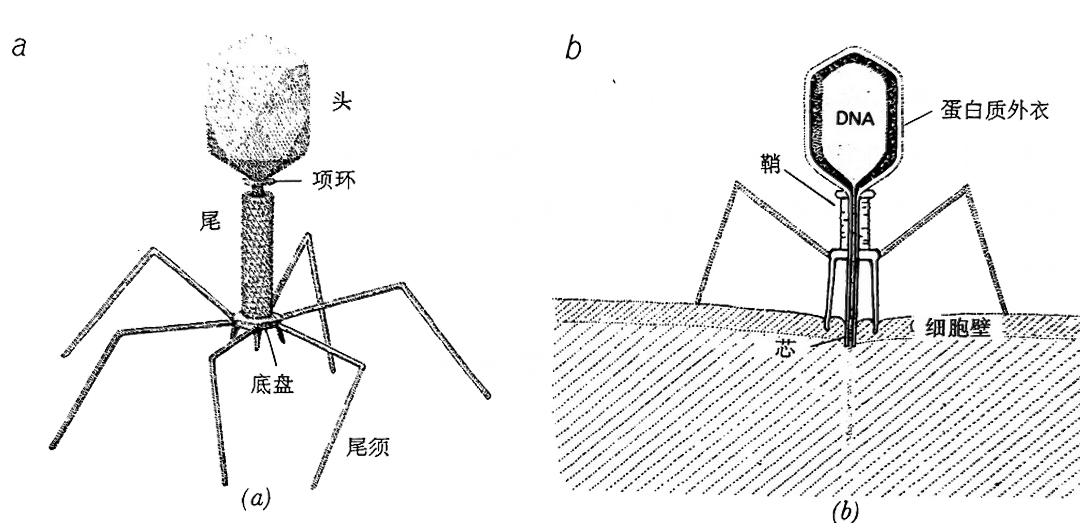
\includegraphics{img_101.png}
\caption[T4细菌病毒。]
  {T4细菌病毒是一个蛋白质聚合体\pnum{a}。它的“头”是形如一种具有三十面的扁长的正十二面体的蛋白质膜,里面充满了DNA,头通过一个颈与尾部相连。尾部是包在一个可收缩的鞘内的空心芯子,安在四周有六条须根、下面有若干钉子的底盘上。钉子和须根使病毒牢牢地粘在细菌的细胞壁上\pnum{b}。鞘的收缩使芯子穿透细胞壁,病毒的DNA进入细胞。[选自哈那瓦尔特和海因斯,《生命的化学基础》,第230页。]}
\end{figure}

我们来考虑生物学家特别宠爱的一种细胞:大肠杆菌细胞,以及生物学家特别宠爱的入侵这种细胞的家伙:凶恶可怕的T4噬菌体,其形状如\fig{101}。这种神奇的小东西看上去有点像登月舱和蚊子的混血儿,可它却比蚊子凶得多。它有一个“头”,里面储存着它的全部“知识”——即它的DNA;它有六条“腿”,以便抓牢它选定入侵的细胞;它有一个像蚊子那样的“刺针”(叫“剌尾”可能更合适些)。主要的区别是,蚊子利用它的刺针来吸血,而T4噬菌体则利用它的剌针违背它的牺牲品的意志,把自己的遗传物质强行注入细胞。所以噬菌体在那个小小的天地里犯有“强奸”罪。

\section{分子特洛伊木马}

病毒DNA进入细胞后会发生什么事呢?按拟人的说法,病毒“希望”它的DNA能得到与宿主细胞的DNA完全相同的待遇。这就意味着要能被转录和被翻译,于是就使它可以指挥合成它自己的特殊的、与宿主细胞相异的蛋白质,然后这些蛋白质就开始各司其职。这相当于利用“密码”(即遗传密码)秘密地把外来蛋白质输送到宿主细胞中,然后再来“解码”(制造它们)。在某种意义上,这很像特洛伊木马的故事:数百名战士藏进一个看上去无害的巨大木马,当他们进城之后,就钻出来占领城市。这些异己的蛋白质一旦从它们的载体DNA中被“翻译”出来(合成出来),就投入行动。

\begin{figure}
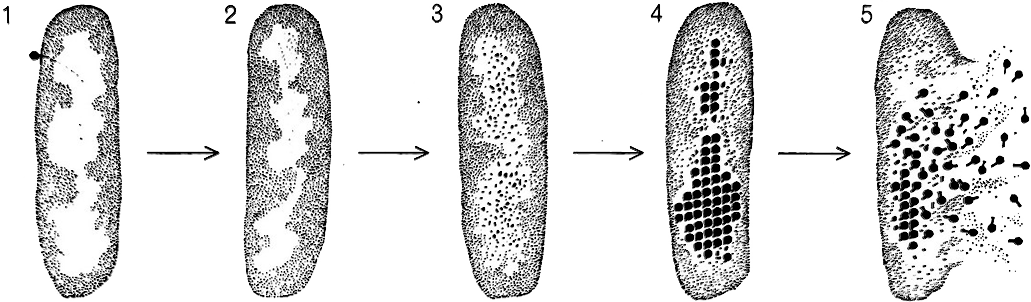
\includegraphics{img_102.png}
\caption[细菌受到病毒的感染。]
  {当病毒的DNA进入细菌之后,病毒感染就开始了。细菌的DNA被瓦解,而病毒的DNA得到复制。病毒结构蛋白的合成以及它们装配成病毒的过程一直在继续,直到撑破细胞,释放出微粒为止。[选自哈那瓦尔特和海因斯,《生命的化学基础》,第230页。]}
\end{figure}

由噬菌体T4所指挥的一系列行为已得到仔细研究,差不多是如下所述(也见\fig{102}和\fig{103}):

\thisfloatsetup{capbesidesep=mqquad}
\begin{figure}
\fcapside[\FBwidth]{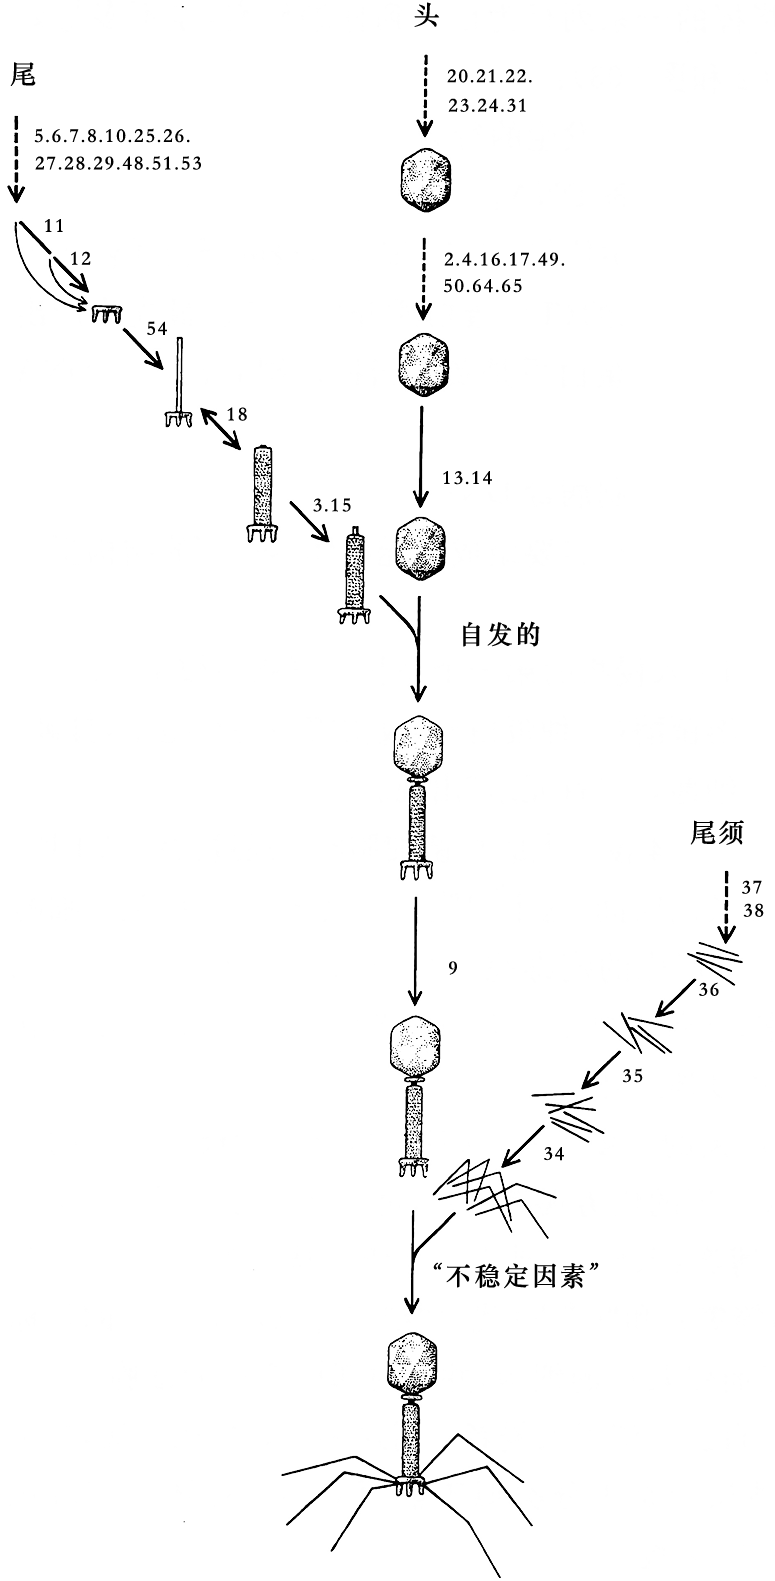
\includegraphics[width=!,height=\textheight]{img_103.png}}{%
\caption[T4病毒的形态发生。]
  {T4病毒的形态发生通道有三个主分支,分别形成头、尾和尾须,然后结合起来形成完整的病毒微粒。[选自哈那瓦尔特和海凶斯,《生命的化学基础》,第237页。]}}
\end{figure}

\begin{longtabu}[c]{cX}
\toprule
\endfirsthead
\multicolumn2r{\small\kaishu(续表)}\\
\midrule
\endhead
\midrule
\endfoot
\bottomrule
\endlastfoot
发生时刻 & 发生的行为 \\*
\midrule
第0分 & 注入病毒DNA。 \\
第1分 & 破坏了主体的DNA。细胞本身的蛋白质停止生产,异己的(T4)蛋白质开始生产。最先生产出的一批蛋白质是负责指挥复制异己(T4)DNA的。\strut \\
第5分 & 开始复制病毒DNA \\
第8分 & 开始生产将要组成新噬菌体“躯体”的结构蛋白。 \\
第13分 & T4入侵物的第一个完整的复制品被生产出来。 \\
第25分 & 溶菌酶(一种蛋白质)攻击寄主的细胞壁,打破细菌,“二百元组”出现。\strut\\
\end{longtabu}

这样,当噬菌体T4侵入大肠杆菌细胞时,经过大约二十四五分钟这样一段不长的时间,这个细胞就完全被颠覆、撕裂。啪的一下,大约二百个与原先的病毒完全相同的复制品——“二百元组”——跑了出来,准备去攻击更多的细菌细胞,而原先的细胞在这个过程中被大幅度地毁坏。

尽管从一个细菌的角度来看,这种事情是一种极为严重的威胁,但从我们的大尺度的优劣观点来看,可以把它看成两名对手之间的一种娱乐性博弈:入侵者,或T方(依照病毒的T偶数族命名,包括T2,T4,等等),和“C”方(代表“细胞”[Cell])。T方的目标是:为了复制自己而侵入C的细胞,并从内部接管C的细胞。C方的目标则是:保护自己并消灭入侵者。用这种方式描述的话,分子TC-博弈可以被认为是十分类似于前面对话中描述的宏观龟[Tortoise]蟹[Crab]之战。

\section{识别、伪装、标识}

这种“博弈”强调了一个事实:识别过程是细胞和亚细胞生物学的中心主题。分子(或一些高层结构)如何互相识别?为了做到这一点,酶必须能锁在其基质的特殊“拴缚部位”上,细菌必须能区别它自己的DNA和噬菌体的DNA,两个细胞必须能通过一种有控制的方式彼此识别和相互作用。这种识别问题可能会使你想起当初关于形式系统的那个关键问题:你怎么才能说清一个符号串有没有某种性质(比方说“是定理”)?有没有一个判定过程?这类问题并不限于数理逻辑:它还渗入计算机科学乃至(我们已经看到了)分子生物学。

对话中描述的那种标识技术,实际上就是大肠杆菌智斗噬菌体入侵者的计策。其思想是:DNA串能通过一种化学手段来标识,即把一个小分子——甲基——排在各种核苷酸上。这种标识操作并不改变DNA的正常生物性质,换句话说,甲基化(标识了的)的DNA能够转录得和未甲基化(未标识的)的DNA一样,所以它仍然能指挥蛋白质的合成。但是,如果主体细胞有某些特殊机制能检验DNA是否有标识,那么这种标识就会是非常重要的了。具体地说,主体细胞可能有一个酶系统来搜寻未加标识的DNA,而且只要找到这样的DNA就毫不留情地把它砍碎破坏掉。此刻,呜呼哀哉的是所有未加标识的入侵者。

核苷酸上甲基标识可以比作一个书法流派的特征。利用这种比喻,我们可以说大肠杆菌细胞在寻找以其“本派字体”——即与它自己特征一致的书法——写下的DNA,并砍掉以“异端”书法写下的一切DNA。当然,噬菌体的反策略则是学会标识自己,从而哄骗那些它们打算侵入的细胞来复制自己。

这种TC之战一类的博奕可以继续到任意复杂的层次,但我们不再继续了。基本的事实是:这是一场力图排斥全部入侵者的主体细胞与力图把自己的DNA渗入宿主细胞、并使它把这个DNA转录成mRNA(从而保证它的复制)的噬菌体之间的战斗。任何一种成功地获得这种自复制方法的病毒DNA,都可以说是具有这样一种高层次的解释:“我可以在X型细胞内被复制。”一定要把这与早先谈到的、在进化论上没有什么意义的那种噬菌体区别开来。早先谈的那种噬菌体是给破坏自己的那些蛋白质编码,其高层解释则是一个自戕句子:“我不能在X型细胞内被复制。”

\section{汉肯句子与病毒}

分子生物学中这两种互为对照的自指类型,在数理逻辑中都有对应的东西。我们讨论过自戕噬菌体的类比物——哥德尔型的符号串,它断言自己在特定的形式系统中不可制造。此外,我们还可做出一个与实际噬菌体相应的句子:该噬菌体断言了它自己在特定的细胞内可以生成。这样的句子就是断言它自己在特定形式系统中可以生成。这类句子被冠以数理逻辑学家列昂·汉肯的名字,称作汉肯句子。可以严格顺着哥德尔句子的线路去构造它们,唯一的不同是丢掉一个否定号。当然,还得从一个“服”号串开始:
\[
\exists a:\exists a':<"TNT-PROOF-PAIR"\{a, a'\}∧"ARITHMOQUINE"\{a'',a'\}>
\]
然后利用标准的手段继续下去,令上述“服”号串的哥德尔数是$h$,于是就对这个“服”号串作算术㧟摁,从而得到一个汉肯句子:
\begin{multline*}
\exists a:\exists a':<"TNT-PROOF-PAIR"\{a, a'\}∧\\
  "ARITHMOQUINE"\{\underbrace{SSS\dotsc SSS}_{\text{$h$个$S$}}0/a'',a'\}>
\end{multline*}
\lnote{(顺便说一句,你能看出这个句子与~G的不同点吗?)}我明白地把它写出来,是为了指出:汉肯句子并没有给它自己的推导开出完整的处方,它只是断言存在一个推导。你可能对它的断定能不能得到验证深感怀疑。汉肯句子真有推导吗?它们的确像它们自己宣称的那样是个定理吗?想一下下面的情形是会有所帮助的:人们怎么会相信一个自称“一贯正确”的“死亡研究专家”呢——他可能正确,但也可能不正确。汉肯句子就比那种专家更靠得住吗?如果那种专家对你说:“其实,人都会死于饭前洗手”,你相信吗?

已经证明,这些汉肯句子一律都讲的是真话。理由并不显然,不过我们将不加证明地接受这一使人奇怪的事实。

\section{隐式汉肯句子之别于显式汉肯句子}

刚才说了,一个汉肯句子对于它自己的推导过程并没说出什么,只是断言有那么一个推导存在。现在,就有可能发明出汉肯句子这一主题的一个变奏——明确描述了自己的推导过程的句子。这种句子的高层解释就不是“存在某个符号串序列是我的推导”,而是“此处描述的符号串序列……是我的推导。”我们把前一种句型叫隐性汉肯句子,而把这种新型的句子称作显性汉肯句子,因为它们显式地描述了自己的推导。应当注意的是,显性汉肯句子与其隐性的弟兄们不同,它们不一定是定理。事实上,很容易写出一个符号串,它断言自己的推导由单个符号串$0=0$组成,但这是个假句子,因为$0=0$不是任何东西的推导。不过,也可以写出一个是定理的显性汉肯句子——即事实上给出它自己的推导方案的句子。

\section{汉肯句子和自组装}

我之所以要区分显性和隐性汉肯句子,是因为这很好地对应着两类病毒之间的一个重要的区别。有一类病毒(比如所谓的“烟草花叶病毒”),叫做自组装病毒;同时也还有另一类病毒,比如我们最喜欢用的T偶数族病毒,叫做非自组装病毒。区别何在?这可以直接类比于隐性和显性的汉肯句子。

一个自组装病毒的DNA只给新病毒的各个部分编了码,而不给任何酶编码。一旦这些部分都造了出来,那个诡秘的病毒就依靠它们自行连接起来,而毋需什么酶的帮助。这样的过程依赖于各个部分在细胞的醇厚饮料中游泳时彼此之间所具有的化学亲和力。不光是病毒,某些细胞器——例如核糖体——也是自组装的。有些时候可能也需要酶——不过在这种情形,酶是从宿主细胞中硬拉来为其所奴役的,这就是自组装的含义所在。

反之,诸如T偶数号那样的比较复杂的病毒的DNA,就不仅给各个部分编码,而且也给在各部分组装成整体的过程中起特殊作用的各种酶编码。由于这个组装过程不是自发的而是需要“一些装置”,所以这些病毒不能看作是自组装。自组装元件与非自组装元件之间的区别,从本质上讲就是:前者不必告诉细胞任何有关它们结构的事情,就安然完成自复制,而后者则需要给出一些有关如何组装它们自己的指令。

这样一来,与隐性汉肯句子和显性汉肯句子相平行的东西也就非常清楚了。隐性汉肯句子是自证明的,但关于它们的证明却什么也没说出来——它们类似于自组装病毒;显性汉肯句子指示了自己证明的构造——这类似于在复制自己的过程中指挥主体细胞的那些比较复杂的病毒。

像病毒这样复杂的自组装生物结构的概念,会使我们想到建造复杂的自组装机器的可能性。设想有这样一系列的零部件,当把它们放入一个适当的背景环境中时,就能通过某种方式自动地集合起来形成一台复杂的机器。这似乎不着边际,实际上却是描述烟草花叶病毒依靠自组装来进行自复制的过程的一种精确方式。有机体(或机器)的整个构造的信息,散布在它的各个部分之中,而不是集中在某一个地方。

这个概念还能引导我们走向一个奇怪的方向,如在《一位烟民富于启发性的思想》中所看到的那样。在那里,我们看到螃蟹如何利用这样一种思想:自组装信息可以四下散开,而不集中在一处。他希望这能防止他的唱机毁于乌龟的破坏手段。不幸的是,正像那些最最精致的公理模式一样,一旦这个系统建立起来并“梳理”完毕,它的良定义性就使它要受到一个足够聪明的“哥德尔化算子”的攻击,而这就是螃蟹所讲的那些令人伤心的故事。尽管看起来荒唐,对话中异想天开情节的与现实的距离并不那么遥远,它就存在于陌生的、梦幻般的细胞世界之中。

\section{两个突出的问题:分化与形态发生}

这样,自组装可以是构造细胞的某些子单元以及某些病毒的手段——可是构造那些极为复杂的宏观结构——比如大象或蜘蛛的躯体,或者维氏捕蝇草——的手段是什么呢?归巢的本能是怎样在鸟的脑子中建立起来的?追猎的本能又是如何在狗的脑子里建立的?简言之,DNA如果仅仅能指挥在细胞中合成一些蛋白质,它又怎么能如此惊人准确地控制宏观生物的严格结构和功能呢?这里主要有两个不同的问题。一个是细胞分化的问题:如何区分具有同样的DNA却又扮演不同角色的细胞——例如肾细胞、骨髓细胞、脑细胞?另一个是形态发生的问题(“形体的出生”):局部水平上的细胞间的相互作用,如何导致大规模的、总体的结构和组织——诸如身体的各个器官、面貌、脑的各个部位等等?尽管我们现在对细胞的分化和形态发生都还知之甚少,但看起来这种手段是存在于细胞内部和细胞之间非常协调的反馈和“前馈”机制之中的,这种机制通知细胞何时“启动”何时“停止”各种蛋白质的生产过程。

\section{反馈和前馈}

在细胞中,如果所需要的某种物质太多了或太少了,就会发生反馈,那时细胞就得用某种方式调整组装这种物质的生产线。前馈也涉及对组装线的调整,不过不是根据当时最终产物的总量,而是根据该组装线的某些“已出厂的产品”的总量。有两种主要方式实现否定性的前馈或反馈。一种方法是阻止有关的酶起作用——也就是说“堵住”它们的活性部位。这叫做抑制。另一种方法是干脆不让有关的酶产生!这叫做阻遏。从概念上讲,抑制比较简单:只须堵住组装线上第一个酶的活性部位,整个合成过程就要停下来。

\section{阻遏物和诱导物}

阻遏则比较诡秘。一个细胞如何阻止一个基因,不让它被表示出来呢?回答是:细胞使这个基因转录不出来。这意味着它必须阻止RNA聚合酶开展工作。顺着DNA的长线,恰好在细胞不想转录的那个基因面前的通道中设置一个巨大的障碍物,就可以达到这个目的。这种障碍物是有的,叫做阻遏物。阻遏物本身也是蛋白质,而且它们能拴在DNA上特定的放置障碍物的部位,这种部位(我弄不清为什么)叫做操纵基因。于是,一个操纵基因就是对紧挨在它后面的基因进行控制的部位,它后面的基因则称为操纵子。由于在实现一个长的化学变化的过程中,是一系列的酶在一齐发生作用,所以它们经常是一个挨一个地编码的。这就说明了为什么一个操纵子常常含有几个基因而不只是一个。成功地阻遏一个操纵子,产生的效果是这一系列基因都得不到转录,这意味着会有一大批酶都处于未合成的状态。

肯定性的前馈和反馈又怎么样呢?仍有两种可能:\pnum{1}释放受阻的酶,\pnum{2}停止对有关操纵子的阻遏。(应当注意到大自然多么喜欢双重否定!这可能有着十分深刻的道理。)使阻遏受到阻遏的机制要用到一类分子,称为诱导物。诱导物的作用很简单:它在一个阻遏蛋白有机会拴在DNA分子的某个操纵基因上之前,与这个阻遏蛋白结合起来。这样得到的“阻遏物与诱导物复合体”就不可能拴在一个操纵基因上,于是就为把联着的操纵子转录到mRNA上,然后再翻译成蛋白质打开了方便之门。通常,最终的产品或某些“已出厂产品”可以起诱导物的作用。

\section{反馈与怪圈的对比}

话说到这里,让我们来区别一下抑制和阻遏这类过程中的简单型反馈,和中心法则映射中所展示的不同信息层次之间的怪圈。在某种意义上讲,两者都是“反馈”,但后者要比前者深刻得多。当诸如色氨酸或异亮氨酸这样的一个氨基酸(以诱导物的形式)拴住它的阻遏物起着反馈作用,从而使其更多的副本得以制造的时候,它并没有说出如何构造它自己。它只是通知酶去制造那些副本。这可以与收音机的音量作个比较。当声音注入听者的耳朵时,有可能导致人去减小或增大音量本身。但这与广播本身命令你打开或关掉收音机——或者要你调到另一个波长上,或者,甚至是教你如何组装另一台收音机——相比,是完全不同的两码事!后面的这些事更像是各种不同的信息层次之间的那种兜圈子。因为此时收音机信号中的信息被“解码”并翻译成心智上的结构。收音机的信号是一些符号构成物,是这些符号的意义在起作用——这时是使用,而非谈论。另一方面,当声音太响时,这些符号就不是在传达意义。它们只被看作很响的声音,因而等于没有意义——这时是谈论,而非使用。这种情形就更像蛋白质调整其合成速率所使用的反馈圈子了。

两个相邻的、具有完全相同的基因类型、但有不同功能的细胞之间的区别,在于它们的基因组中的不同节段受到阻遏,因而它们的蛋白质工作点不同,这已经形成理论了。这样的假说可以解释人体的不同器官中细胞何以会有显著的差别。

\section{分化的两个简单例子}

从初始的细胞开始,一遍又一遍地复制,造出大量各种各样的、具有特定功能的细胞的过程,可以比做一种在人们之间传送连锁信的过程。其中每个新的参加者都得忠实地传达消息,但都要加一点润色。最后就会得到很多彼此相差极大的书信。

对这种分化思想给出另一种说明的,是下面这种与分化型自复制相似的极为简单的计算机。设想一个很短的、被一个双向开关控制的程序,程序中有一个内部参数$N$——一个自然数。这个程序能按两种方式运行——向上方式和向下方式。当按照向上方式运行时,它把自己复制到该机器的存储器的邻近部位,不过它的“女儿”的内部参数是原先的$N$加上$1$。当按照向下方式运行时,它不做自复制,而是计算数值
\[
\frac{(-1)^N}{2N+1}
\]
然后把它加到前面运行过程中所得的总数上。

好了,假定一开始存储器中有一份这个程序,其中的$N=0$,状态为“向上”。那么该程序就要在存储器里相邻部位中复制自己,并使$N=1$。重复这个过程,新程序又要在与自己相邻处复制自己,得到$N=2$的副本。就这样一遍一遍地重复下去……所发生的事是一个很大的程序在存储器中膨胀。存储器装满后,过程就停止了。可以看成是整个存储器中装满了一个大程序,它含有很多彼此相似但却是分化了的模块——或叫“细胞”。如果此刻把程式开关扳到“向下”,并运行这个大程序,那会发生什么呢?首先第一个“细胞”运行起来,算出$1/1$。接着第二个“细胞”运行,算出$-1/3$,并和前面的结果相加,然后第三个“细胞”运行,算出$1/5$,并与前面的和相加……最终的结果是整个“组织”——那个大程序——算出大量(与存储器内能装下的“细胞”一样多)的项的和:
\[
1-\frac13+\frac15-\frac17+\frac19-\frac1{11}+\frac1{13}-\frac1{15}+\dotsb
\]

由于这个级数收敛(尽管很慢)于$\uppi/4$,所以我们就有了一个“表现型”的东西,它的功能是计算一个著名的数学常数的值。

\section{细胞中的层次混合}

我希望,对诸如标识、自组装、分化、形态发生、以及转录和翻译等过程的描述,能有助于描述一个十分复杂的系统,那就是细胞——一种面貌全新的信息加工系统。在中心法则映射中,我们已经看到,尽管可以试着在程序和数据之间划一条分界线,但这种区别多少有些随意。按这种思路再进一步,我们就会发现,不仅程序和数据犬牙交错,就是程序的解释程序以及实际的处理机、乃至语言,都是如此紧密相关的。尽管(在一定程度上)有可能给各层次划定边界,把它们分开,但是认识到各层次之间的交叉、混合也同样重要——而且同样吸引人。在生物系统中一个令人惊讶的事实说明了这一点:为做到自复制而必需的所有因素(即:语言、程序、数据、解释程序及处理机)高度协同动作,以致于到了能把它们同时复制出来的程度——这表明生物的自复制比人类沿这些方向所设计的任何东西都深奥得多。例如本章开头所列出的自复制程序,就得假定事先存在三个客观的方面:语言,解释程序和处理机,而且并不复制它们。

我们来试着用计算机科学的术语总结一下给细胞的各个子单元分类的各种方法。先看DNA。由于DNA包含着构造作为该细胞的活性物质的各种蛋白质的全部信息,所以可以把DNA看成是用一种高层语言写出、随后又被翻译(或解释)成细胞“机器语言”的一个程序。另一方面,DNA本身又是受各种酶操纵的被动的分子,在这个意义上,DNA分子又恰像一长段数据。第三,DNA包含着能生成tRNA“单词卡片”的模板,这意味着DNA也含有它自己的高层语言的定义。

我们转向蛋白质。蛋白质是活性分子,并执行细胞的全部功能,所以,把它们看成用“细胞的机器语言”写成的程序(细胞本身做为处理机)就十分合适。另一方面,由于蛋白质是硬件,而大多数程序是软件,所以把蛋白质看成处理机也许更好一些。第三,蛋白质经常受到其它蛋白质的作用,这意味着蛋白质经常是数据。最后,还可以把蛋白质看作解释程序,这时是把DNA看成一组高级语言程序,在这种情形中,酶只是在执行DNA密码写下的程序,也就是说蛋白质起解释程序的作用。

还有核糖体及tRNA分子。它们是从DNA到蛋白质的翻译媒介,这种翻译可以比拟成一个程序从高级语言到机器语言的翻译过程。换句话说,核糖体有解释程序的功用,而tRNA分子规定了高级语言的定义。不过,对这个翻译过程还有一种看法:核糖体是处理机而tRNA是解释程序。

分析全部这些生物分子之间的相互关系时,我们还只是蜻蜓点水而已。所看到的是,我们倾向于认为有明显区别的那些层次,被大自然十分惬意的混合在了一起。实际上,在计算机科学中,已经有着把一个信息处理系统中看上去不同的所有方面混为一谈的明显趋势。人工智能的研究尤其如此,而人工智能的研究通常是站在计算机语言设计的最前沿。

\section{生命的起源}

了解了这些难以置信的、复杂的、相互联结的软件和硬件玩意儿,会使人提出一个自然而又基本的问题:“它们怎么开始的呢?”这倒真是一件令人困惑的事情。我们不得不设想有一个“揪鞋带举自己”的过程,这有点像开发新计算机语言时使用的那个过程——可是从简单分子到整个细胞的“揪鞋带”简直超出了我们的想象力。有许多关于生命起源的理论,它们遇到下述这个最最关键的问题时都不灵了:“遗传密码及其翻译机能(核糖体和tRNA分子)都是如何发生的?”目前,我们不得不满足于一种惊奇和敬畏的感觉,这不是一个答案带来的满足。也许体味这种惊奇和敬畏比有一个答案更令人满意——至少暂时是这样。
